\section{Systematic uncertainties} % (fold)
\label{sec:systematic_uncertainties}

The following sections cover the suite of systematic uncertainties on the measurement that has been considered. All uncertainties are summarised in Section~\ref{sub:summary_of_systematic_uncertainties}.

\subsection{Strong phase uncertainties} % (fold)
\label{sub:strong_phase_uncertainties}
\begin{figure}[tp]
    \centering
    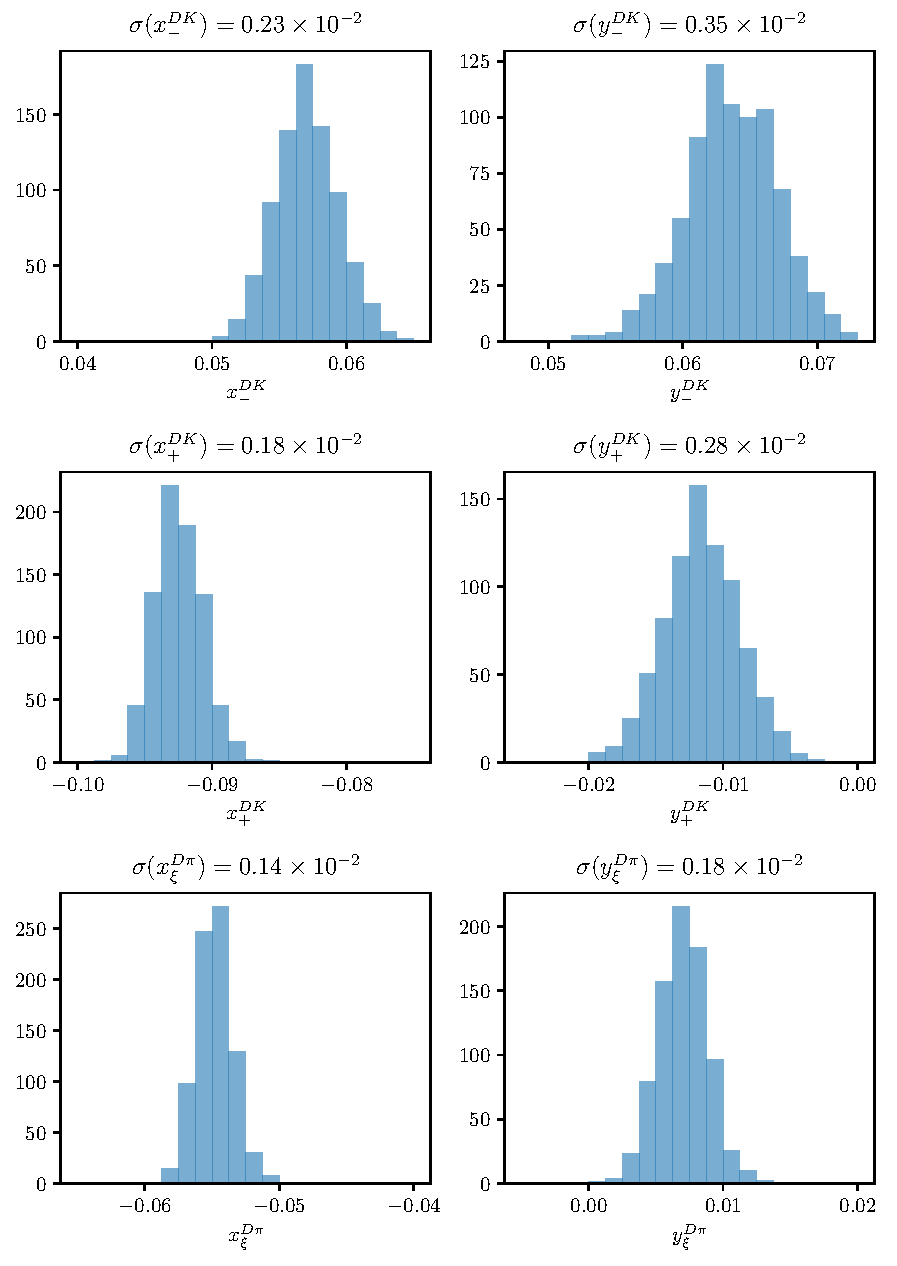
\includegraphics[width=0.7\columnwidth]{figures/analysis/systematics/strong_phase_variation.pdf}
    \caption{Spread of central values for the fitted observables when the input \ci and \si from the BESIII+CLEO combination are varied according to their uncertainties and correlations. 
    %The default fit values are shown with the dotted lines.
    }
    \label{fig:cisi_variation}
\end{figure}
The observables \xpmdk, \ypmdk, \xxidpi and \yxidpi are extracted using the central values of \ci and \si from the BESIII--CLEO combinations~\cite{CLEOCISI,BESCISI,BESCISIKSKK}. Subsequently, the measurement uncertainty on these inputs is propagated to the observables by performing a large set of fits to data, using alternative values of $c_i$ and $s_i$. The new $c_i$ and $s_i$ values are obtained by smearing the central values by their measured statistical and systematic uncertainties while taking into account their correlations. 
The use of different $c_i$ and $s_i$ values changes the extracted \xpmdk, \ypmdk, \xxidpi and \yxidpi values. The width of the distributions of central values extracted from 1000 data fits are assigned as a systematic uncertainty. The distributions are shown in Fig.~\ref{fig:cisi_variation} and the assigned uncertainties are summarised in Table~\ref{tab:cisi_syst_corr_matrix}. The correlation matrix related to the strong-phase uncertainty can be obtained from the correlations observed between observables in the fits, and is also given in the table. 

The set of $(\ci, \si)$ that was employed in this analysis will be used in a series of future BPGGSZ measurements, both with additional \B decay modes within the \lhcb collaboration and by the Belle~II collaboration. This introduces some correlation between the measurement results. In order to allow for an estimate of the degree of correlation by future analysts, the 1000 samples $(\ci,\si)$ values and the corresponding fit results for $(\xpmdk, \ypmdk, \xxidpi, \yxidpi)$ have been made public as supplementary material to Ref.~\cite{GGSZ-B2Dh}.

\begin{table}[tb]
\centering
\caption{Systematic uncertainties and correlation matrix due to strong-phase inputs. 
\label{tab:cisi_syst_corr_matrix}}


% autogenerated via 06_systematics/cisi_related/StrongPhase%20uncertainties.ipynb
\begin{tabular}{l|cccccc}
\toprule
\multicolumn{7}{c}{Uncertainty $(\times 10^{-2})$}\\ \midrule
 & $x_-^{DK}$ & $y_-^{DK}$ & $x_+^{DK}$ &$ y_+^{DK}$ & $x_\xi^{\D\pi}$ &$ y_\xi^{\D\pi} $\\
\midrule
$\sigma$ & $0.23$ & $0.35$ & $0.18$ & $0.28$ & $0.14$ & $0.18$ \\
\bottomrule \multicolumn{7}{c}{} \\
\multicolumn{7}{c}{Correlations}\\ \midrule
 &$ x_-^{DK}$ & $y_-^{DK}$ & $x_+^{DK}$ &$ y_+^{DK}$ & $x_\xi^{\D\pi}$ &$ y_\xi^{\D\pi} $\\
\midrule
$x_-^{\DK} $    & $\phantom{-}1.000$ & $-0.047$ & $-0.490$ & $\phantom{-}0.322$ & $\phantom{-}0.189$ & $\phantom{-}0.144$ \\
$y_-^{\DK} $    &    & $\phantom{-}1.000$ & $\phantom{-}0.059$ & $-0.237$ & $-0.116$ & $-0.117$ \\
$x_+^{\DK} $    & &       & $\phantom{-}1.000$ & $\phantom{-}0.061$ & $\phantom{-}0.004$ & $-0.139$ \\
$y_+^{\DK} $    & & &          & $\phantom{-}1.000$ & $\phantom{-}0.127$ & $-0.199$ \\
$x_\xi^{\Dpi}$ & & &     &         & $\phantom{-}1.000$ & $\phantom{-}0.638$ \\
$y_\xi^{\Dpi}$ & & &     &    &         & $\phantom{-}1.000$ \\
\bottomrule
\end{tabular}  

\end{table}




% subsection strong_phase_uncertainties (end)

\subsection{Efficiency-profile-related systematic uncertainties} % (fold)
\label{sub:efficiency_profile_related_systematic_uncertainties}

The non-trivial efficiency profile over the Dalitz plot can have a range of effects, considered in the sections below.

% subsection efficiency_profile_related_systematic_uncertainties (end)

\subsubsection{The assumption that \texorpdfstring{$\eta^{\D\kaon}(\sm, \sp) = \eta^{\D\pi}(\sm, \sp)$}{etaDK = etaDpi}}

The assumption that $\eta^{\D\kaon}(\sm, \sp) = \eta^{\D\pi}(\sm, \sp)$ was examined in detail in Section~\ref{sub:efficiency_profile_over_the_dalitz_plot}. It was found that with signal yields similar to those in the data set, no statistically significant difference between the efficiency profiles $\eta^{\D\kaon}(\sm, \sp)$  and $\eta^{\D\pi}(\sm, \sp)$ was discernible, and no additional uncertainty due to this assumption is assigned.

\subsubsection{The assumption that \texorpdfstring{$\eta(\sm, \sp)$}{eta(s-,s+)} = \texorpdfstring{$\eta(\sp, \sm)$}{eta(s+,s-)}}
\label{subs:eta_symmetry}


The measurement is sensitive to effects that break the assumption $\eta(\sm, \sp)=\eta(\sp, \sm)$. Such a breakdown would mean that opposite points on the Dalitz plot have different efficiencies and can only arise through a charge detection asymmetry (e.g that it is more likely to detect a $K^+$ in the detector rather than a $K^-$.)\footnote{Note that the measurement is insensitive to any asymmetry in the reconstruction of the companion track.}
%There are two possible sources of such an asymmetry. The first is that due to the curvature of the tracks the region of the detector traversed by positive tracks is different to that traversed by negative tracks. If these regions of the detector have different performances then we end up with a charge asymmetry. However the reversal in magnet polarity switches the regions of detector traversed and hence any variation in tracking performance across the tracking stations is averaged out. Secondly there are differences in the matter interactions between $K^+$ and $K^-$. For this reason the asymmetry is expected to be larger for kaons (and hence \KsKK) than it is for pions (\KsPiPi). 

\begin{figure}[tp]
    \centering
    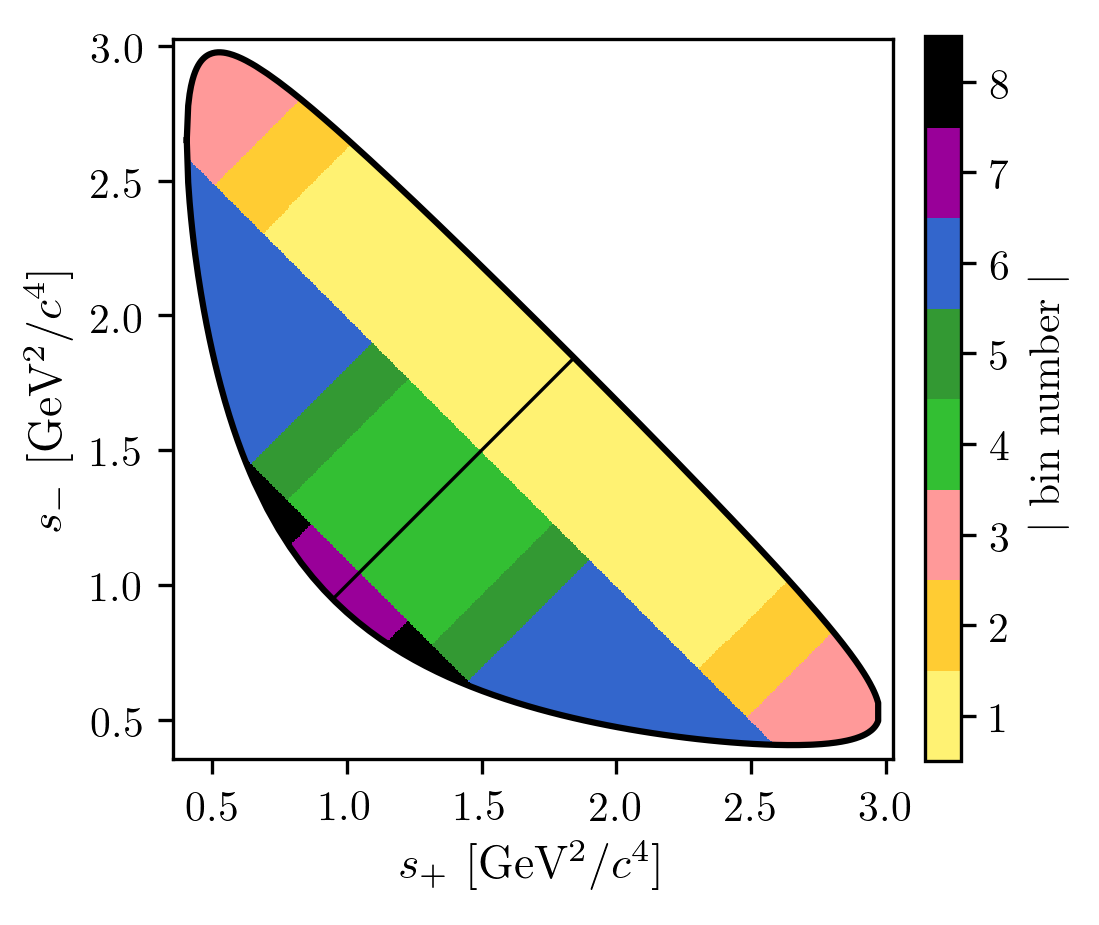
\includegraphics[width=0.45\columnwidth]{figures/theory/binnings/KsPiPi_rect.png}
    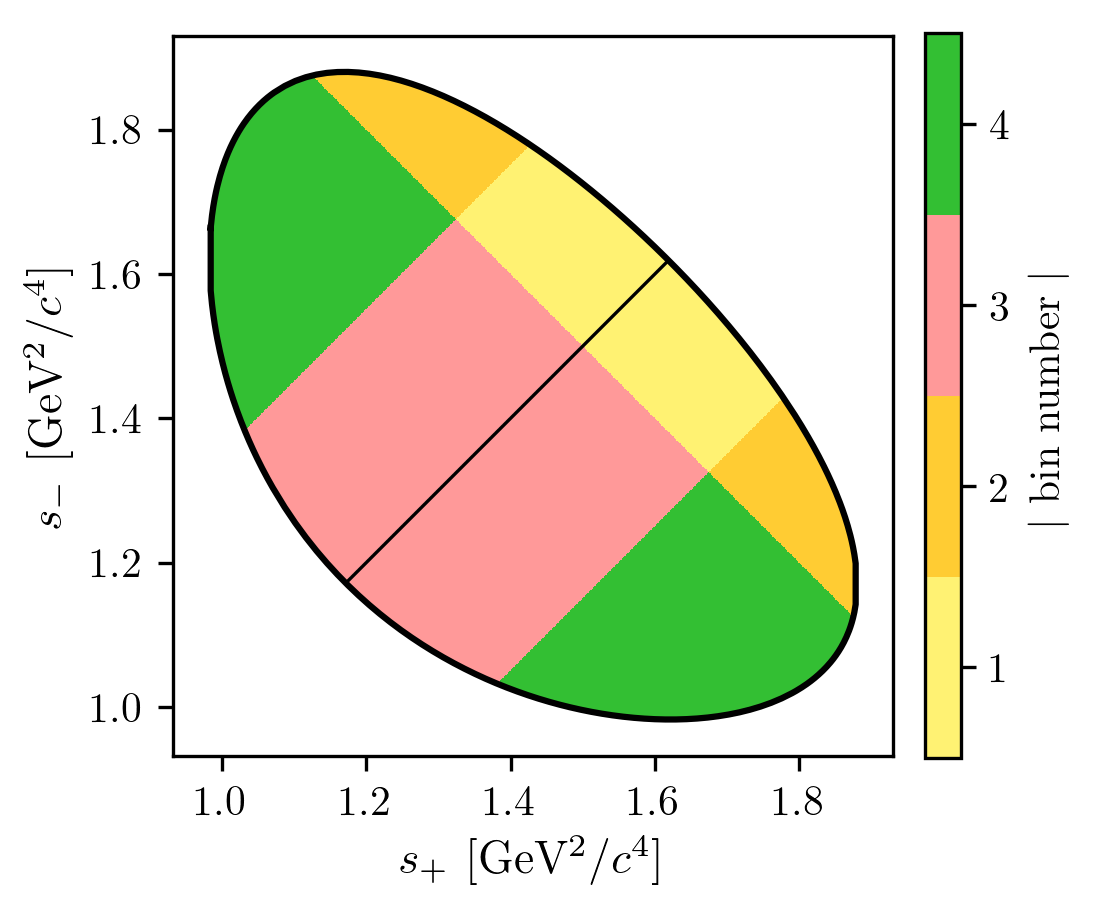
\includegraphics[width=0.45\columnwidth]{figures/theory/binnings/KsKK_rect.png}
    \caption{The rectangular binning schemes used to group candidates in (left) the \DtoKspipi and (right) the \DtoKsKK categories in a number of systematic uncertainty studies.}
    \label{fig:rect_bins}
\end{figure}

The potential size size of such an asymmetry can be studied in simulation where the \D decay has a uniform distribution over the allowed phase space; in such simulated samples, it would manifest itself as an observation different fractional yields 
of $B^-$ decays in bin $i$ and $B^+$ decays in bin $-i$. This effect has been looked for using the large samples of \BtoDpi decays that were generated for the analysis of 2015 and 2016 data. The study is performed using the rectangular binning schemes shown in Fig.~\ref{fig:rect_bins}, because this scheme is most sensitive to effects that vary smoothly over phase space. The comparison plots are shown in Fig.~\ref{fig:efficiency_symmetry_check}, where it can be seen that the $p$ values for the hypothesis that there is no asymmetry all take on reasonable values. Hence no further systematic uncertainty is considered.

\begin{figure}[tb]
    \centering
    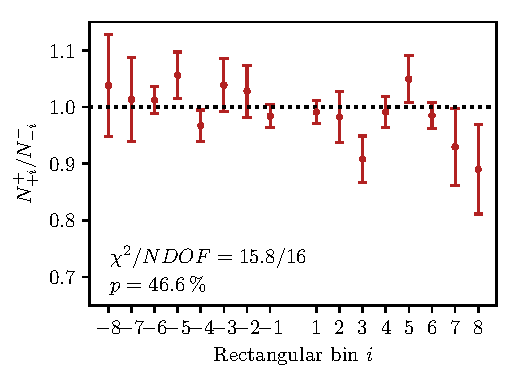
\includegraphics[width=0.45\columnwidth]{figures/analysis/systematics/efficiency_symmetry_Pi_PiPi_LL.pdf}
    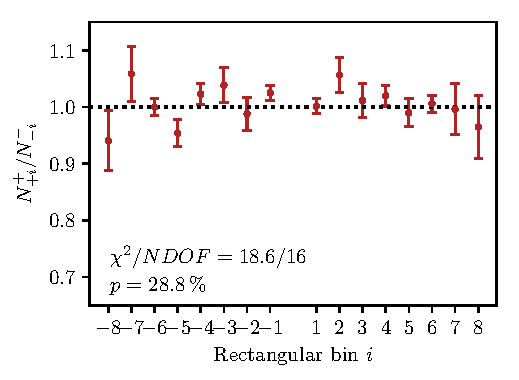
\includegraphics[width=0.45\columnwidth]{figures/analysis/systematics/efficiency_symmetry_Pi_PiPi_DD.pdf}
    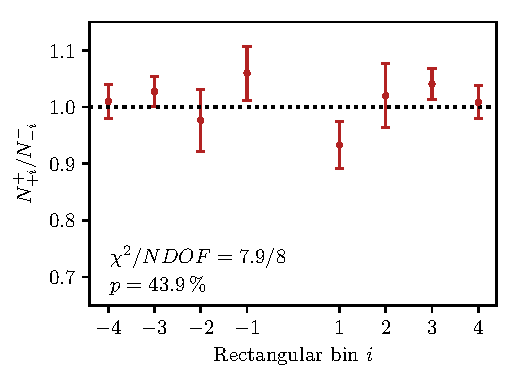
\includegraphics[width=0.45\columnwidth]{figures/analysis/systematics/efficiency_symmetry_Pi_KK_LL.pdf}
    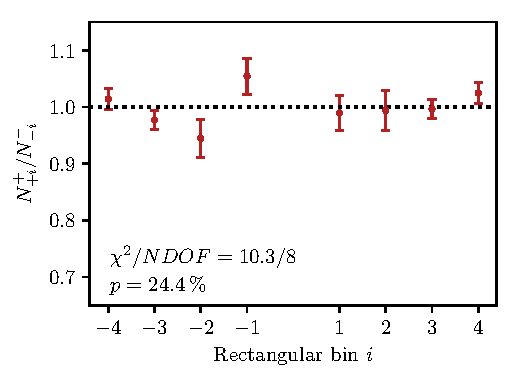
\includegraphics[width=0.45\columnwidth]{figures/analysis/systematics/efficiency_symmetry_Pi_KK_DD.pdf}
    \caption{Comparison of the ratio of \Bp decays reconstructed in bin $+i$ to \Bm decays reconstructed in bin $-i$ for simulated \BtoDpi decays where (top) \DtoKspp and (bottom) \DtoKskk, also split into (left) the LL and (right) the DD categories, using the rectangular binning schemes in Fig.~\ref{fig:rect_bins}. Calculated $p$ values for the hypothesis that the ratio is flat are also shown, all of them being at least 20\,\%.}
    \label{fig:efficiency_symmetry_check}
\end{figure}



\subsubsection{\texorpdfstring{Effect of phase-space efficiency profile on \ci and \si}
{Effect of phase-space efficiency profile on ci and si}} % (fold)
\label{ssub:texorpdfstring_effect_of_phase_space_efficiency_profile_on_ci_and_si}

% subsubsection texorpdfstring_effect_of_phase_space_efficiency_profile_on_ci_and_si (end)


As discussed in Section~\ref{sec:strategy_for_lhcb_measurement} there is a small bias, because the \ci and \si values that are used correspond to the definition

\begin{align}\label{eq:ci_si_no_eff}
    \ci = \frac
    {\int_i \text{d}s^2 |\ADS(\smp)||\ADS(\spm)|\cos[\Delta\delta_D(\smp)]}
    {\sqrt{\int_i \text{d}s^2 |\ADS(\smp)|^2}\sqrt{\int_i \text{d}s^2 |\ADS(\spm)|^2}}, \quad (\text{and equivalent for } s_i,)
\end{align}
whereas the non-flat efficiency profile in \lhcb, $\eta(\sm, \sp)\equiv\eta(\smp)$, means that the appropriate \ci' and \si' entering the exact yield expressions are
\begin{align}\label{eq:ci_si_with_eff}
    \ci^\text{eff} = \frac
    {\int_i \text{d}s^2 \eta(\smp)|\ADS(\smp)||\ADS(\spm)|\cos[\Delta\delta_D(\smp)]}
    {\sqrt{\int_i \text{d}s^2 |\ADS(\smp)|^2}\sqrt{\int_i \text{d}s^2 |\ADS(\spm)|^2}}, \quad (\text{and equivalent for } s_i^\text{eff}.)
\end{align}
The shifts $\Delta c_i = c_i^\text{eff}- c_i$, $\Delta s_i = s_i^\text{eff} - s_i$ can be estimated using the efficiency profile in simulation and the latest amplitude models: the 2018 Belle model~\cite{Belle2018} for \DtoKspp and the 2010 BaBar model~\cite{BABAR2010} for \DtoKskk. The strong-phase parameters are first calculated assuming a uniform reconstruction efficiency over phase space according to Eq.~\eqref{eq:ci_si_no_eff}, obtaining a set of values $\{c_i^\text{model}, s_i^\text{model}\}$. Then, an alternative set is calculated, $\{c_i^\text{eff}, s_i^\text{eff}\}$, using the same model, and the reconstruction efficiency profile found in full \lhcb simulation. The results, as well as their differences, are tabulated in Tables~\ref{tab:eff_correction_cisi_d2kspipi}~and~\ref{tab:eff_correction_cisi_d2kskk}. The \lhcb reconstruction efficiency at a given point in phase-space is taken to be proportional to the yield in simulation, as the simulated decays were generated with a uniform distribution over phase space. The efficiency is averaged over the LL and DD categories in the calculation. 

A systematic uncertainty due to employing the measured \ci and \si directly in the fit is assigned by generating a large number of toy data sets where the signal yields are calculated using $(c_i^\text{eff}, s_i^\text{eff})$, and then fitting the data sets using $(c_i^\text{model}, s_i^\text{model})$. The mean bias of each observable in these toys is assigned as the systematic uncertainty, and is determined to be $0.1\times 10^{-2}$ or less for all observables. The smallness of the effect is the reason no effort is made to correct the \ci and \si values in the nominal measurement.


\begin{table}
\centering
    \caption{
    The \ci and \si values for \DtoKspipi decays calculated via the 2018 \belle model~\cite{Belle2018} in two cases: assuming a uniform reconstruction efficiency over phase space, denoted $(c/s)_i^\text{model}$, and including the \lhcb efficiency profile as obtained in simulation, averaged for LL and DD, denoted $(c/s)_i^\text{eff}$. The change due to including the efficiency is also tabulated.
    \label{tab:eff_correction_cisi_d2kspipi}
    }



    % table autogenerated by ANA_scripts/06_systematics/cisi_related/EfficiencyEffectOnCiSi.ipynb
    \begin{tabular}{c|ccc|ccc}
    \toprule
    Bin & 
    $c_i^\text{model}$ & $c_i^\text{eff}$ & $\Delta c_i$ &
    $s_i^\text{model}$ & $s_i^\text{eff}$ & $\Delta s_i$ \\
    \midrule
    1 & $           -0.027$ & $           -0.007$ & $\phantom{-} 0.019$ & $\phantom{-} 0.812$ & $\phantom{-} 0.794$ & $           -0.018$ \\
2 & $\phantom{-} 0.837$ & $\phantom{-} 0.859$ & $\phantom{-} 0.022$ & $\phantom{-} 0.164$ & $\phantom{-} 0.152$ & $           -0.012$ \\
3 & $\phantom{-} 0.163$ & $\phantom{-} 0.163$ & $           -0.000$ & $\phantom{-} 0.872$ & $\phantom{-} 0.880$ & $\phantom{-} 0.008$ \\
4 & $           -0.914$ & $           -0.915$ & $           -0.001$ & $\phantom{-} 0.076$ & $\phantom{-} 0.082$ & $\phantom{-} 0.006$ \\
5 & $           -0.149$ & $           -0.170$ & $           -0.021$ & $           -0.856$ & $           -0.854$ & $\phantom{-} 0.002$ \\
6 & $\phantom{-} 0.373$ & $\phantom{-} 0.362$ & $           -0.011$ & $           -0.782$ & $           -0.805$ & $           -0.023$ \\
7 & $\phantom{-} 0.863$ & $\phantom{-} 0.862$ & $           -0.000$ & $           -0.203$ & $           -0.202$ & $\phantom{-} 0.002$ \\
8 & $\phantom{-} 0.860$ & $\phantom{-} 0.862$ & $\phantom{-} 0.002$ & $\phantom{-} 0.330$ & $\phantom{-} 0.336$ & $\phantom{-} 0.006$ \\

    \bottomrule
    \end{tabular}


\end{table}
\begin{table}
\centering
    \caption{
    The \ci and \si values for \DtoKskk decays calculated via the 2010 \babar model~\cite{BABAR2010} in two cases: assuming a uniform reconstruction efficiency over phase space, denoted $(c/s)_i^\text{model}$, and including the \lhcb efficiency profile as obtained in simulation, averaged for LL and DD, denoted $(c/s)_i^\text{eff}$. The change due to including the efficiency is also tabulated.
    \label{tab:eff_correction_cisi_d2kskk}
    }



    % table autogenerated by ANA_scripts/06_systematics/cisi_related/EfficiencyEffectOnCiSi.ipynb
    \begin{tabular}{c|ccc|ccc}
    \toprule
    Bin & 
    $c_i^\text{model}$ & $c_i^\text{eff}$ & $\Delta c_i$ &
    $s_i^\text{model}$ & $s_i^\text{eff}$ & $\Delta s_i$ \\
    \midrule
    1 & $\phantom{-} 0.738$ & $\phantom{-} 0.735$ & $           -0.002$ & $\phantom{-} 0.266$ & $\phantom{-} 0.263$ & $           -0.003$ \\
2 & $           -0.697$ & $           -0.744$ & $           -0.046$ & $\phantom{-} 0.332$ & $\phantom{-} 0.329$ & $           -0.003$ \\

    \bottomrule
    \end{tabular}



\end{table}

% subsection strong_phase_related_uncertainties (end)



\subsection{Mass shapes} % (fold)
\label{sub:systematics_from_mass_shapes}


A number of uncertainties relate to the mass distributions that enter the fit model. Each is described in detail the sections below.

\subsubsection{Determination of shape parameters} % (fold)
\label{ssub:determination_of_shape_parameters}

The statistical uncertainties on the shape parameters that are obtained in fits to simulated decays and in the first stage fit to data need to be propagated to the uncertainty on the obtained parameters. This is done via a bootstrapping procedure, repeating these steps many times:
\begin{itemize}
    \item Each of the data sets used determine parameters of the signal, crossfeed, and lowmass shapes that are fixed in the first-stage fit to data of Section~\ref{sec:signal_and_background_components} are re-sampled with replacement, drawing a number of events equal to the original data-set size. These are from simulation for signal and lowmass shapes, and real data for the crossfeed shapes. All of the shapes are fit again, on the re-sampled data sets.
    \item The real dataset is re-sampled with replacement, drawing a number of events equal to the original data-set size. Then, the first-stage fit of Section~\ref{sec:signal_and_background_components} is repeated with the shapes obtained as described above, obtaining values for the remaining shape parameters.
    \item Finally, the \CP fit is repeated using the shape parameters determined in the preceding steps, but \emph{without} re-sampling the dataset (to avoid a statistical spread in the obtained central values that is independent of the shape parameters).
\end{itemize}
The uncertainty on each observable is taken to be the standard deviation of the set of central values obtained as described above. This procedure propagates the statistical uncertainty on the fixed parameters to the observables, in a way that takes correlations into account, and which does not rely on the uncertainty estimates in the preliminary fits being accurate. The uncertainties are less than $0.1\times 10^{-2}$ for all \DK observables, in line with earlier analyses, and less than $0.2\times 10^{-2}$ for all \Dpi observables.

% There is also a potential systematic uncertainty on the obtained mass shapes. For the case of signal, this arises due to imperfections in simulation, leading to the shape fit to MC decays not providing exactly the right shape. We assess the potential impact, by determining alternative signal shape parameters in a fit to MC with an extra tight truth-matching cut of $\texttt{BKGCAT==0}$; ie. to a simulation sample that \emph{we know} does not represent the shape in data well. This leads to much worse pulls in the fit to data than the default shape, as exemplified in Fig.~\ref{fig:alt_signal_shape_bkgcat}, but has a completely negligible impact on the central values obtained for the \CP-violation observables. Hence we do not consider a further systematic due to this effect.

% \begin{figure}[tb]
%     \centering
%     % 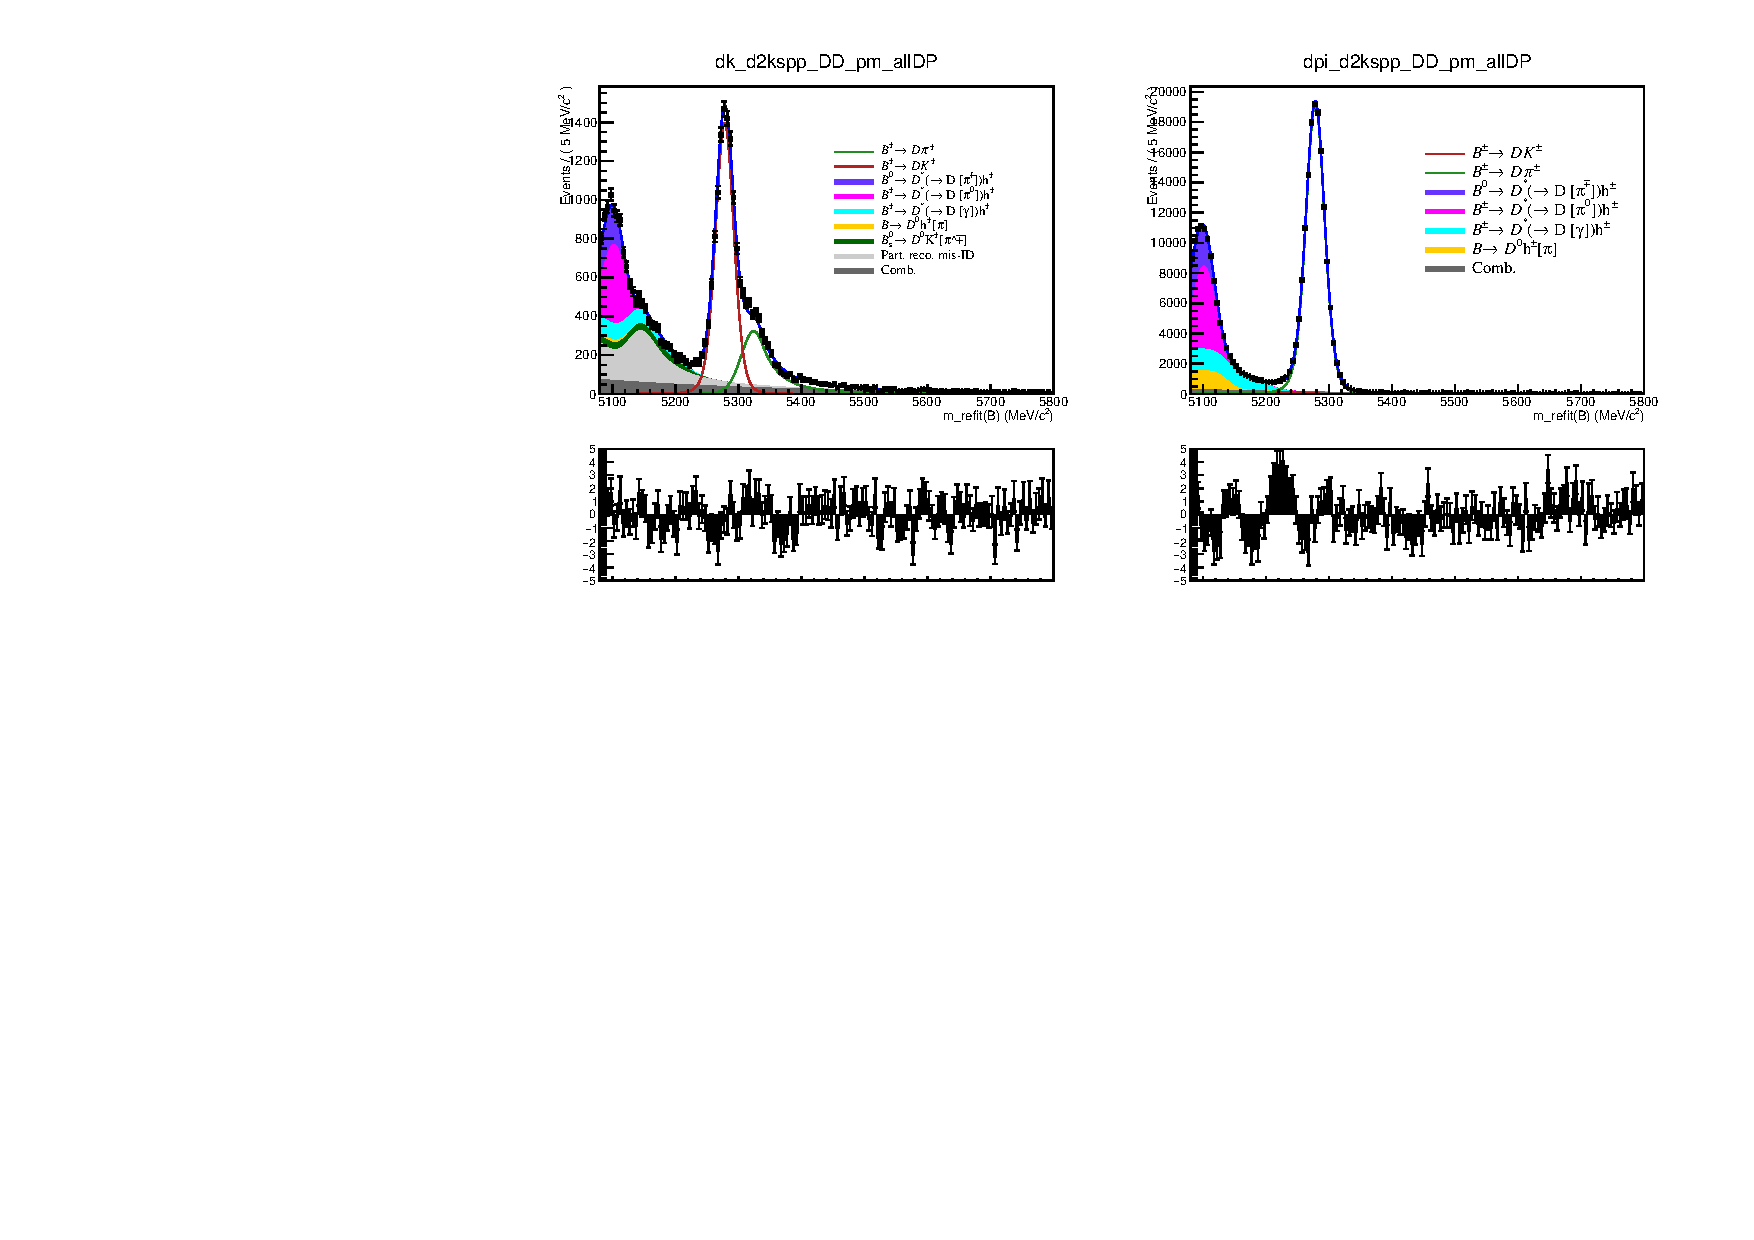
\includegraphics[width=0.8\columnwidth]{figs/systematics/plots/d2kspp_DD_alt_BKGCAT_signal_shape_fit.pdf}
%     \caption{Example of a fit to $\BtoDh$ decays in the DD category where \DtoKspipi, where the signal tail parameters were fit in a simulation sample with a truth matching cut of $\texttt{BKGCAT==0}$. The pulls are much worse than for the default fit to data, but the binned fit obtains essentially the same central values for the \CP-violation observables.}
%     \label{fig:alt_signal_shape_bkgcat}
% \end{figure}

A potential bias arises due the use of sWeights when obtaining the mass distribution of decays where a $\pi\leftrightarrow \kaon$ misidentification has taken place. This is because the $m_\mathrm{swap}(\D h^\pm)$ mass that is calculated while assuming a swapped companion hypothesis and the nominal $m_\mathrm{default}(\D h^\pm)$ mass are correlated (it is always the case that $m_\mathrm{swap} > m_\mathrm{default}$ for a $\pi\to\kaon$ misidentification ,for example). Thus, the assumptions of the sPlot method are not satisfied~\cite{sPlot}. The correlation coefficient in the signal region is about 20\,\% for simulated signal decays. In order to assess the potential impact, an alternative mass distribution for $(\BtoDpi)\to(\BtoDK)$ cross-feed is derived that does not rely on sWeights. Instead of fitting \BtoDpi sample in the whole fit range and assigning sWeights before recalculating the \B mass under the kaon companion hypothesis, the shape is obtained using \BtoDpi candidates in the signal region. This is possible because the \BtoDpi sample is very pure. The shapes are compared in Fig.~\ref{fig:compare_alt_noSW_misID_shapes} and are seen to be almost identical. Thus the sWeights do successfully subtract the contribution of combinatorial and partially reconstructed backgrounds in the default setup. The impact on the obtained \CP-violation observables of using one or the other shape in the fits is negligible, and no further systematic uncertainty is assigned due to this effect. 

\begin{figure}[tp]
    \centering
    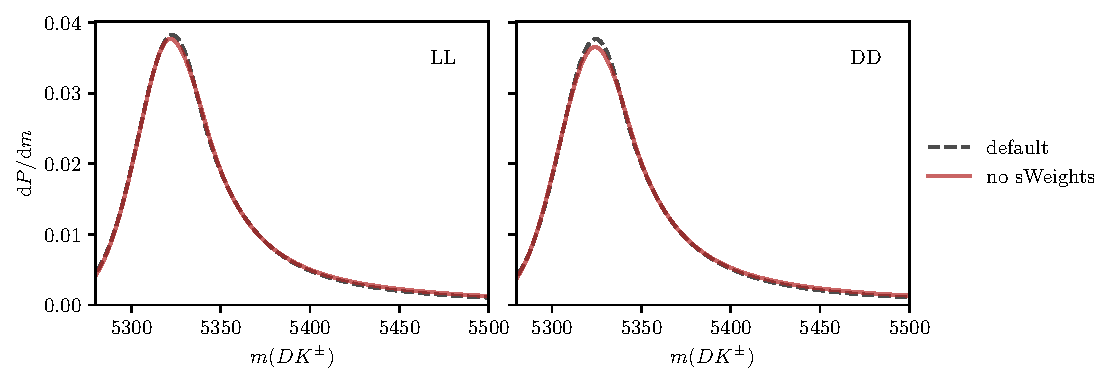
\includegraphics[width=0.85\columnwidth]{figures/analysis/systematics/misID_sW.pdf}
    \caption{Comparison of the default and no-sWeights alternative shape for the $\D\pi\to\D\kaon$ cross-feed component in the (left) LL and (right) DD categories where \DtoKspipi. The binned fit obtains essentially the same central values for the \CP-violation observables, independently of which shape is used. }
    \label{fig:compare_alt_noSW_misID_shapes}
\end{figure}


% subsubsection determination_of_shape_parameters (end)

\subsubsection{Using the same mass shapes in all Dalitz bins} % (fold)
\label{ssub:using_the_same_signal_shape_in_all_dalitz_bins}

The mass shapes obtained the first-stage fit where all Dalitz bins are combined, are used in each individual bin of the subsequent binned fit. However, there could be some variation in the shape over the \D-decay phase space, due to correlations between the phase-space coordinates and particle kinematics. The potential effect is investigated in pseudoexperiments, where toy data sets are generated with alternative signal, crossfeed, and combinatorial-background shapes that are allowed to differ between bins, and fitted with the default shapes. The partially reconstructed background is treated in a separate study, because further physics effects contribute to bin-by-bin variation, as described in the following section. 

The alternative signal and cross-feed mass shapes are fitted independently in each bin, following identical procedures to those outlined in Sections~\ref{sub:signal_decays}~and~\ref{sub:texorpdfstring_cross_feed_between_btodh_channels}. Examples of the obtained shapes are compared in Figs.~\ref{fig:signal_bin_by_bin}~and~\ref{fig:misID_bin_by_bin}.

\begin{figure}[tp]
    \centering
    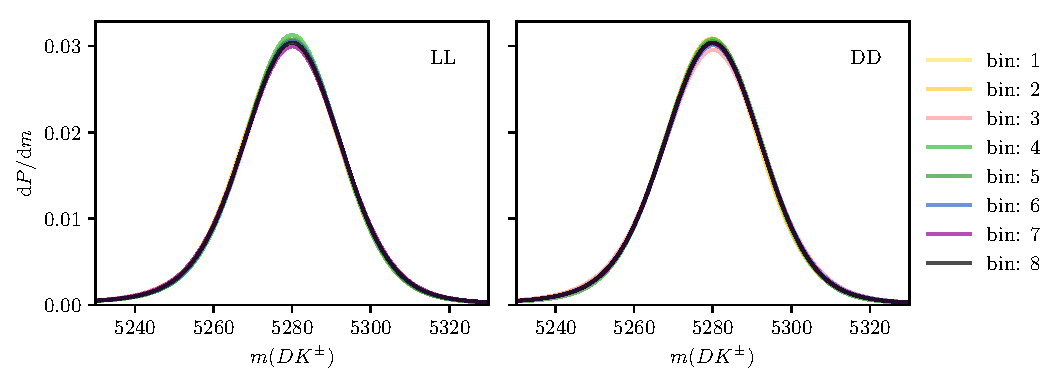
\includegraphics[width=0.85\columnwidth]{figures/analysis/systematics/signal_bin_by_bin.pdf}
    \caption{Signal shapes obtained in fits simulated \BtoDpi decays for individual Dalitz bins in the optimal binning scheme, for (left) LL and (right) DD candidates in the \BtoDpiDtoKspipi category. }
    \label{fig:signal_bin_by_bin}
\end{figure}

\begin{figure}[tp]
    \centering
    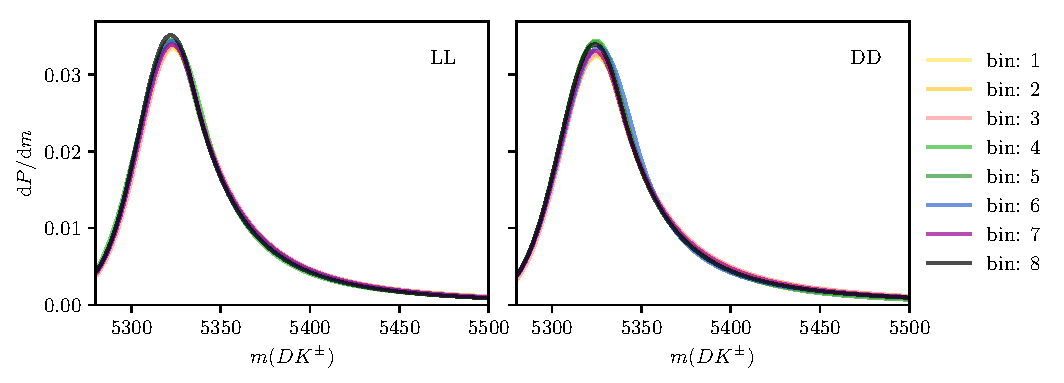
\includegraphics[width=0.85\columnwidth]{figures/analysis/systematics/misID_bin_by_bin.pdf}
    \caption{Mass shapes for $\D\pi \to\D\kaon$ cross feed obtained for individual Dalitz bins in the optimal binning scheme, for (left) LL and (right) DD candidates in the \DtoKspipi category.}
    \label{fig:misID_bin_by_bin}
\end{figure}

The shape of the combinatorial background can also vary over the \D decay phase-space; for example will the relative amount of fake \D candidates versus real \D decays paired with a random bachelor certainly depend on the real \D decay amplitude for a given phase-space region. The effect is investigated in the high \B-mass sideband $m_\B\in[5600, 6500]\mevcc$, in which the $m(\D h^\pm)$ distribution is fitted with a single exponential distribution, in bins of the Dalitz plot. The fits combine \Bp and \Bm candidates and merge bins $+i$ and $-i$, and are carried out for both the \emph{optimal} binning scheme of Fig.~\ref{fig:kspipi_bins} (on page~\pageref{fig:kspipi_bins}) and a \emph{rectangular} binning scheme, shown in Fig.~\ref{fig:rect_bins}, which better captures continuous trends over the Dalitz plot. The study is done for \DtoKspipi only due to available statistics. The DD category of \BtoDpi decays has the largest statistics and shows the largest variation, and the fitted slopes for this channel are shown in Fig.~\ref{fig:comb_sloped_single_channel}. Two effects are visible: 1) there is some variation in the slope as a function of the Dalitz bin, especially visible for the rectangular scheme, and 2) the exponential slope is larger in general in the high \B-mass sideband. The latter effect does not pose a problem, since the employed exponential is found to provide an excellent fit in the default fit region. It does however need to be taken into account when when deriving alternative, bin-dependent combinatorial slopes relevant for the default fit region. In order to do so, the alternative slope for bin $i$ is defined
\begin{align}
    \alpha^i_\mathrm{default-range} = \frac{\alpha^i_{\mathrm{high-}m_\B}}{\alpha^{all-DP}_{\mathrm{high-}m_\B}}\times \alpha^{all-DP}_\mathrm{default-range},
\end{align}
and used when generating the combinatorial-background component of the toy data sets for the study.


\begin{figure}[tbp]
    \centering
    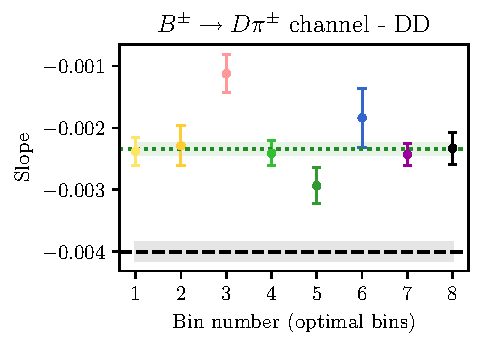
\includegraphics[width=0.47\columnwidth]{figures/analysis/systematics/comb_slopes/com_slopes_by_bin_dpi_DD.pdf}
    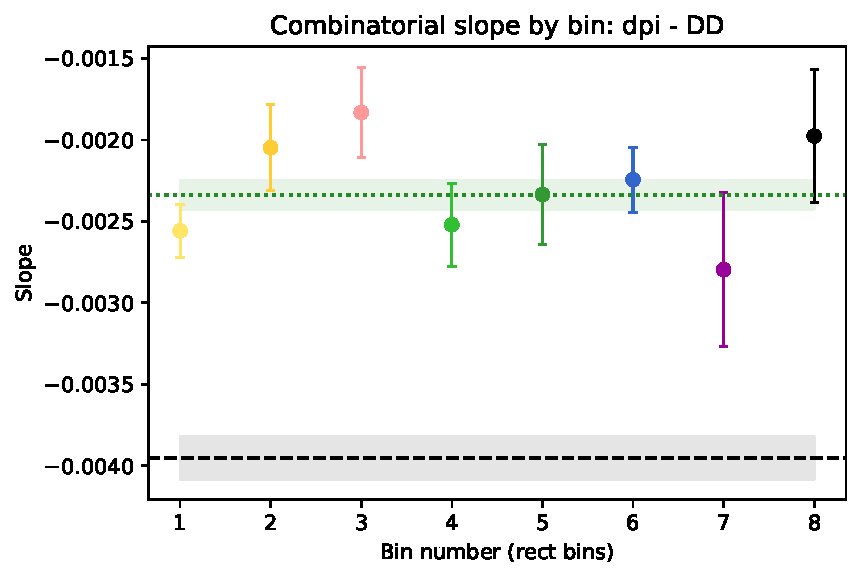
\includegraphics[width=0.47\columnwidth]{figures/analysis/systematics/comb_slopes/com_slopes_by_bin_dpi_DD_rect.pdf}
    \caption{Plot of (dots) combinatorial slope in the high \B mass background for each bin in the (left) the optimal binning scheme and (right) the rectangular binning scheme, for the DD \BtoDpiDtoKspipi category. The slope when all bins are combined (green, dashed line) is also shown, and compared with (black dashed line) the slope in the default fit region. }
    \label{fig:comb_sloped_single_channel}
\end{figure}




%The obtained mass shapes are compared in Fig. \toadd{add and comment}. 
The average bias obtained for for each observable in the ensemble of pseudoexperiments is assigned as a systematic uncertainty, found to be about $0.1\times 10^{-2}$ for each observable. 

% subsubsection using_the_same_mis_id_shape_in_all_dalitz_bins (end)

\subsubsection{Ignoring physics effects in the lowmass background} % (fold)
\label{ssub:using_the_same_part_reco_shape_in_all_dalitz_bins_ignoring_physics_effects_in_the_lowmass_background}

In the \CP fit, the same relative fractions of partly reconstructed \Bpm and \Bz backgrounds are used in each bin, as determined in the first-stage fit described in Section~\ref{sec:signal_and_background_components} (whereas the partly reconstructed $\Bs\to\Dzb[\pi^+]K^-$ background is treated separately). However the distribution over the Dalitz plot depends on whether the partly reconstructed decays occur via an intermediate \Dz meson, a \Dzb meson, or and admixture of both. Consider a decay reconstructed as $\Bm\to\D\Km$ but which is actually a partially-reconstructed background. There are then four types of background that should be considered:
\begin{itemize}
\item Decays in which the \PD-meson in the true decay is a \Dz-meson. An example of this is $\Bm\to\Dstarz(\Dz\piz)\pim$ for which the \piz from the \Dstarz decay is missed and the \pim is misidentified as the companion \Km. These are denoted '\Dz-like'.\footnote{The naming convention is defined in terms of the \D present in candidates reconstructed as \Bm decays. For the charge conjugate case this decay would of course happen via a \Dzb, but is still denoted \Dz-like.}

\item Decays in which the \PD-meson in the true decay is a \Dzb-meson. An example of this is $\Bs\to\Dzb\pip\Km$ for which the \pip is missed and the \Km is reconstructed as the companion \Km. These are denoted '\Dzb-like'.

\item Decays in which the \PD meson in the true decay can be either flavour, and both \D flavours contribute to the decay amplitude. An example of this is $\Bm\to\Dstar\Km$ for which the total decay amplitude into a \D final state has contributions from both \Dstarz (decaying to \Dz) and \Dstarzb (decaying to \Dzb). The relative amplitude magnitude and phase between the two possible \PB decays are denoted $r_{B}^{D^*}$ and $\delta_{B}^{D^*}$ respectively. These are denoted  `$r_B$-like'. %The best-fit values from UTFit are 0.118 and $-51^\circ$ respectively. (We assume any \CP violation in the previous two bullet points is negligible, which is a good approximation.)

\item Decays that can be reconstructed as both \Dz- and \Dzb-like but where there is no quantum-mechanical interference. An example is $\Bzb\to\Dz\pip\pim$ decays where either the \pip or \pim can be reconstructed as the bachelor. These are denoted 50/50 \Dz-like and \Dzb-like. 

\end{itemize}
For $\Bp\to DK^+$ decays everything is CP conjugated. The Dalitz-plot distribution for each of these cases is:
\begin{itemize}
\item \Dz decays (`\Dz-like')
\begin{align}
\begin{split}
N_{\pm i}(\Bm) & \propto F_{\pm i} \label{eq:nD0} \\
N_{\pm i}(\Bp) & \propto F_{\mp i}
\end{split}
\end{align}
\item \Dzb decays (`\Dzb-like'):
\begin{align}{}
\begin{split}
N_{\pm i}(\Bm) & \propto F_{\mp i} \\
N_{\pm i}(\Bp) & \propto F_{\pm i}
\end{split}
\end{align}
\item Decays with a quantum-mechanical admixture of \Dz and \Dzb (`$r_B$-like'):
\begin{align}
\begin{split}
N_{\pm i}(\Bm) & \propto F_{\pm i} + (r_{B}^{*})^2\,F_{\mp i} + 2\sqrt{F_{+i}F_{-i}}[x_{-}^{*}c_{\pm i} + y_{-}^{*}s_{\pm i}] \\
N_{\pm i}(\Bp) & \propto F_{\mp i} + (r_{B}^{*})^2\,F_{\pm i} + 2\sqrt{F_{+i}F_{-i}}[x_{+}^{*}c_{\pm i} - y_{+}^{*}s_{\pm i}] \label{eq:nrB} 
\end{split}
\end{align}
where $(x_{\pm}^{*},y_{\pm}^{*})$ are defined analogously to the standard \BtoDK case.

\item 50/50 \Dz-like and \Dzb-like:
\begin{align}
\begin{split}
N_{\pm i}(\Bm) & \propto F_{\pm i} + F_{\mp i}  \\
N_{\pm i}(\Bp) & \propto F_{\pm i} + F_{\mp i}  \label{eq:n5050} 
\end{split}
\end{align}
\end{itemize}
The use of a single background shape across all bins may therefore introduce biases because, if an admixture of these backgrounds is present, such a shape has no sensitivity to bin-to-bin variations. 

% various fractions calculated in ANA_scripts/06_systematics/shape_related/LowmassPhysicsEffects.ipynb
In the $\D\pi$ channel, the dominant backgrounds are all \Dz-like ($\Bzb\to\Dstarm\piz$, $\Bm\to\Dz\rho^-$, $\Bm\to\Dstarz\pim$). There is a small contribution from $\Bzb\to\Dz\rho(\to\pip\pim)$ decays where either the \pip or \pim from the \rhoz decay can be assigned as the bachelor, and thus this background is 50/50 \Dz-like and \Dzb-like. The background only corresponds to about 0.5\,\% of the total partially reconstructed background and thus the impact is small. Nevertheless it is considered in the study described below.

In the \D\kaon channel all categories of background appear. In the mass region of the \CP fit approximately 75.5\% of backgrounds are \Dz-like ($\Bzb\to\Dstarm\Km$, mis-identified $\Bm\to\Dstarz\pim$, and mis-identified $\Bm\to\Dz\rho^-$), 7.5\,\% are \Dzb-like ($\Bs\to\Dzb\pi^+\Km$), 1\,\% is 50/50 \Dz-\Dzb-like (mis-identified \Bz\to\D\rhoz), and 16\% are $r_B$-like ($\Bm\to\Dstar\Km$, $\Bz\to\D\Kstarz$, and $\Bm\to\D\Kstarm$). 

In order to estimate the bias due to ignoring this effect, a large number of toy data sets are generated using the default low mass shapes and total yields from the first-stage fit in Section~\ref{sec:signal_and_background_components}, but distributing each of them individually over the Dalitz-bins according to Eqs.~\eqref{eq:nD0}-\eqref{eq:nrB}. When calculating the distribution of $\Bp\to\Dstarz\Kp$ decays over the Dalitz plot, the values \cite{LHCb-CONF-2018-002}
\begin{align}
    r_B^{D^*} & = 0.191 & \delta_B^{D^*} & = 331.6^\circ
\end{align} are used.  When calculating the distribution of $\Bp\to\Dz\Kstar^+$ decays over the Dalitz plot the values \cite{LHCb-CONF-2018-002}
\begin{align}
        r_B^{K^*} & = 0.092 & \delta_B^{K^*} & = 40^\circ.
\end{align}  are used. The toy data sets are then fit with the default set up, and the observed mean bias assigned as the corresponding uncertainty. The corresponding uncertainties were found to be about $0.1\times 10^{-2}$ for all uncertainties. The variation in the shapes is rather small in the mass range included in the fit, which explains the small impact.

If the \Bs background is \emph{not} treated separately in the default fit, but instead included in a single lowmass background shape along with the \Bz and \Bpm contributions, the systematic uncertainty is an order of magnitude larger when evaluated as described above, and would be a dominating systematic. This motivates the separate treatment of the \Bs background.



% subsection mass_shapes (end)

\subsection{\texorpdfstring{\CP violation and material interaction of the \KS}
{CP violation and material interaction of the KS}} % (fold)
\label{sub:cp_violation_and_material_interaction_of_the_ks}

A systematic uncertainty due to \CP-violation effects and material interaction of the \KS is assigned using the results obtained in Section~\ref{sub:the_impact_on_coupled_btodk_and_btodpi_measurements}. In that section, the expected bias on all observables in a combined \BtoDh measurement was evaluated for the detector geometry and particle kinematics of the \lhcb experiment. The calculation was made for $(r_B^{\DK/\Dpi},\delta_B^{\DK/\Dpi})$ values close to the world averages, and a number of $\gamma$ values; the results were summarised in Fig.~\ref{fig:LHCb_related_biases}. 
The systematic uncertainty is taken to be the largest absolute bias observed for each parameter in the study. The largest uncertainty (on \yxidpi where it is $0.46\times 10^{-2}$) is still an order of magnitude smaller than the statistical uncertainty.
 

% subsection cp_violation_and_material_interaction_of_the_ks (end)

\subsection{Impact of \D mixing} % (fold)
\label{sub:impact_of_d_mixing}

The effect of \D-mixing is not accounted for in the measurement, which leads to a small bias. Earlier studies have shown this to lead to a sub-degree bias on measurements of $\gamma$ in \BtoDK decays, in the case where the \Fi parameters are determined experimentally under the same experimental conditions as the $\gamma$ measurement~\cite{Dmixing}. A number of pseudoexperiments are carried out to verify that this is also the case for the combined \DK--\Dpi setup employed in the thesis. They are performed following the same procedure described in Section~\ref{sub:cp_violation_and_material_interaction_of_the_ks} for the case of \KS\, \CP violation. The yields are calculated while taking \D mixing into account, using the mixing parameter values $x=(0.39^{+0.11}_{-0.12})\,\%$ and $y=(0.65^{+0.06}_{-0.07})\,\%$~\cite{PDG2020}, and then fitted back assuming no \D mixing. The biases are found to be small, as expected, all of them smaller than $0.05\times 10^{-2}$. The largest relative biases are on the \BtoDpi parameters, but even for those the relative effect is less than 2\,\%. In agreement with Ref.~\cite{Dmixing}, it is found that the biases increase with an order of magnitude if the \Fi parameters are fixed to the expected values with no \D-mixing, instead of being determined as part of the fit.

% subsection impact_of_d_mixing (end)
\subsection{PID efficiencies} % (fold)
\label{sub:pid_efficiency_systematic}
The uncertainty related to PID efficiencies is assesses by repeating the full two-stage fit procedure a number of times, each time varying the PID efficiencies within the uncertainties. The used uncertainty includes both a statistical and systematic component, as described in detail in Section~\ref{sub:particle_identification_requirements}. The standard deviations of the central values obtained for each observable are assigned as the systematic uncertainty. The uncertainties come out below $0.1\times 10^{-2}$ for all observables.
% subsection pid_efficiencies (end)

\subsection{Dalitz-coordinate resolution} % (fold)
\label{sub:dalitz_plot_bin_migration}

There is a small systematic uncertainty related to Dalitz-plot-bin migration, where the non-perfect resolution on the momentum measurement means that a candidate is assigned to a different bin that it truly belongs to. This leads to non-negligible net migration between bins that share a border in a region of phase space where the amplitude varies rapidly. However, since the \Fi are measured in the data set, all leading order effects of migration are inherently taken into account. The measurement is only sensitive to differences in migration between the \DK and \Dpi channels and the effect is small. 

The systematic uncertainty due to this effect is assigned using pseudoexperiments. The study is made for the \DtoKspipi mode only, which is sufficient since it completely dominates the overall sensitivity. 
\begin{enumerate}
    \item Signal \BtoDK and \BtoDpi decays are generated continuously over phase space, according to the expected distribution obtained with the latest amplitude model from the Belle collaboration~\cite{Belle2018}, assuming values of $\gamma$ and $(r_B^{\DK/\Dpi},\delta_B^{\DK/\Dpi})$ close to the current world averages.
    \item The Dalitz coordinates of each candidate are then smeared using the experiment resolution obtained in simulation. This is described further below.
    \item Finally, the generated candidates are binned and fitted back using the default setup. 
\end{enumerate}

%This toy generation follows the procedure outlined in Section~\ref{ssub:compare_results_obtained_with_different_binning_schemes}. 

The resolution is obtained via simulation, by comparing the reconstructed phase-space coordinates with those calculated from the true momenta in samples of simulated \DtoKspipi decays. As can be seen in Fig.~\ref{fig:dalitz_coord_resolution_and_correlation}, the resolution is found to vary over phase space and the distribution of shifts has significant exponential tails. In order to take both effects into account, the smearing is done by shifting each generated decay with a realised coordinate shift in full simulation, for a simulated decay that took place at approximately the same place in the Dalitz plot. The shift is multiplied with 120\,\% to take into account that the resolution is generally better in simulation than data. If the shift results in Dalitz coordinates outside the kinematically allowed region, a different shift is applied randomly instead.

The average bias seen in the pseudoexperiments is assigned as the systematic uncertainty. The uncertainties come out at about $(0.1-0.2)\times 10^{-2}$ for all parameters. It is noted that for all four \DK parameters the bias is towards a smaller value of $r_B^{DK}$; this is to be expected, as bin migration washes out the asymmetries in different areas of the Dalitz plot. 

\begin{figure}[tb]
    \centering
    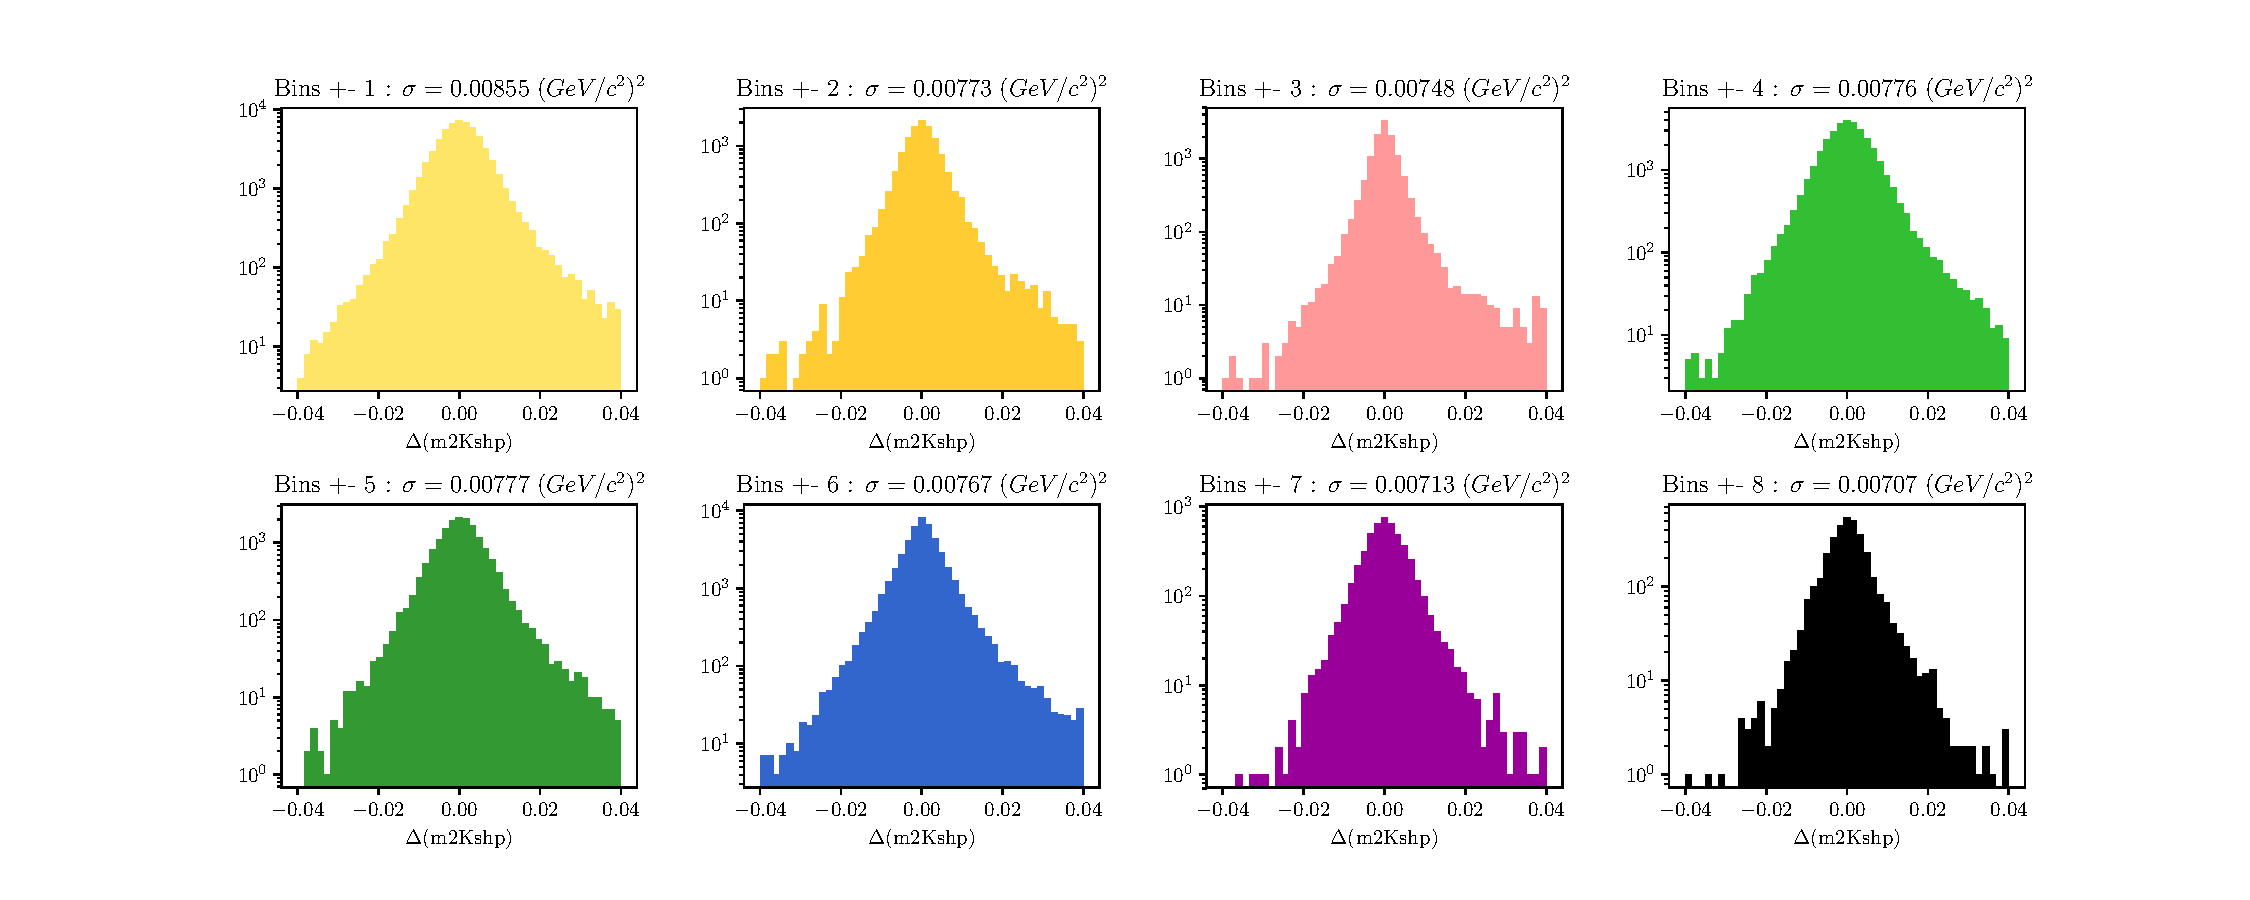
\includegraphics[width=\columnwidth]{figures/analysis/systematics/Dalitz_resolution_rect_bins.pdf}
    \caption{Distribution of the biases $\Delta (m^2) = m^2_{true} - m^2_{reconstructed}$ in simulation for $m^2(\KS \pip)$ in bins of the rectangular binning scheme of Fig.~\ref{fig:rect_bins}.}
    \label{fig:dalitz_coord_resolution_and_correlation}
\end{figure}



\subsection{The fixed yield fractions} % (fold)
\label{sub:the_bs_yield}

A number of relative yields are fixed from efficiencies in simulation and branching fractions. In the \DK modes, this is the case for all the relative yields of the partially reconstructed backgrounds, including partially reconstructed $\B\to\D\pi[X]$ decays where the pion is misidentified as a kaon, and the yield of the $\Bs\to\D\kaon\pi$ background relative to the $\B\to\D\pi$ yield. In the \BtoDpi channel, the only fixed yield ratio is that of the partially reconstructed $\Bpm\to\Dstarz(\to\D\piz)\pipm$ and $\Bz\to\Dstarmp(\to\D\pimp)\pipm$ modes. The uncertainty on the observables due to uncertainties on these fixed fractions is assessed by repeating the two-stage fit procedure many times, each time shifting the yield ratios randomly within their uncertainties. The uncertainty on each observable is taken to be the standard deviation of the set of central values obtained in these fits. These are all smaller than $0.1\times 10^{-2}$.

% The \Bs background is the most dangerous, because it is \Dzb-like and therefore is large in bins where the signal yield is small. Therefore we have investigated the impact of varying the fixed yield fraction of this background further. In Fig.~\ref{fig:Bs_yield_scan} we show the shift in central values of the \BtoDK observables when the yield ratio is varied between 0 and 350\,\%. The background can be seen to lead to a large bias compared to the systematic uncertainties if not treated correctly, and indeed contributes the most to the uncertainty quoted above, but the potential shifts are not large compared to the obtained central values.

\subsection{Systematic uncertainty due to backgrounds that are not modelled in fit} % (fold)
\label{sub:systematic_uncertainty_due_to_backgrounds_that_are_not_modelled_in_fit}

There are a number of backgrounds that are expected to be present at a small level, but which are not modelled in the fits to data because their impact on the fit results is minimal. Instead, a systematic uncertainty is assigned. Each contribution is described in the following sections and the related systematic uncertainties are summarised in Table~\ref{tab:small_backgrounds}.

\begin{table}
    \centering
    \footnotesize
    \caption{Summary of systematic uncertainties due to backgrounds that are potentially present with a small yield, but not included in the mass fit.
    \label{tab:small_backgrounds}}
\begin{tabular}{l|cccccc}
\toprule
\multicolumn{7}{c}{All uncertainties are quoted with implicit: $\times 10^{-2}$} \\
\midrule
Mode & 
$\sigma(x_-^{\DK})$ & $\sigma(y_-^{\DK})$ & 
$\sigma(x_+^{\DK})$ & $\sigma(y_+^{\DK})$ &
$\sigma(x_\xi^{\Dpi})$ & $\sigma(y_\xi^{\Dpi})$ \\
\midrule
$\Lb$ backgrounds                        & 0.04  & 0.05  & 0.04  & 0.06  & 0.08  & 0.13  \\ 
$\B\to\D\mu\nu X$                        & 0.04  & 0.07  & 0.04  & 0.05  & 0.10  & 0.11  \\ 
$\Bpm\to\D(\to \KS \pi \mu \nu) h^\pm$   & 0.00  & 0.03  & 0.02  & 0.02  & 0.00  & 0.00  \\ 
Swapped tracks                           & 0.10  & 0.13  & 0.12  & 0.08  & 0.00  & 0.01  \\ 
\midrule
Total                                    & 0.11  & 0.16  & 0.13  & 0.12  & 0.08  & 0.13  \\ 

\bottomrule
\end{tabular}

\end{table}

% subsection systematic_uncertainty_due_to_backgrounds_that_are_not_modelled_in_fit (end)

\subsubsection{\texorpdfstring{Background from $\Lambda_b$ decays}{Background from Lb decays} } 
\label{sub:background_from_lambda_b_decays}

This section considers the possible impact of the two potential backgrounds from \Lb decays described in Section~\ref{sub:partially_reconstructed_backgrounds}: $\Lb\to\Dz p\pim$  decays where the pion is not included the candidate reconstruction and the proton assigned as the companion, and $\Lb\to\Lc(\to p\KS \pip\pim)\pim$ decays  where a pion in the \Lc decay is not reconstructed and the proton reconstructed as one of the \D decay products. The impact of not including these in the default fit is assessed by generating toy data sets where the backgrounds are included in the generation step, which are then fitted back with default model. The former background is distributed over the Dalitz plot as \Dzb-like, cf. the terminology of Section~\ref{ssub:using_the_same_part_reco_shape_in_all_dalitz_bins_ignoring_physics_effects_in_the_lowmass_background}, since a positive bachelor is produced along with a \Dz meson. The latter is also distributed as \Dzb-like in the study; the exact distribution is unknown, but a \Dzb-like background is likely to have the largest effect and thus this is a conservative choice. The total yields are taken relative to the signal yields, using the yield ratios discussed in Section~\ref{sub:partially_reconstructed_backgrounds}.
The $m(\D h^\pm)$ distributions are obtained using simulated samples, produced with \texttt{RapidSim}. The mean biases come out to be less than $0.1\times 10^{-2}$ for each \CP-violation observable, which is assigned as a systematic uncertainty.

\subsubsection{Semi-leptonic backgrounds} % (fold)
\label{ssub:semi_leptonic_backgrounds_systematic}

The impact of remnant $\B\to\D \mu \nu_\mu$ decays after requiring $\texttt{isMuon=0}$ on the bachelor is assessed in pseudoexperiments. Toy datasets are generated where the background is added in the generation step, which are then fitted with the default model. The background yield relative to  signal and the mass shape are obtained from a sample of fully simulated decays for conditions corresponding to the run conditions in 2012. The obtained bias in the toys is assigned as the systematic uncertainties: it is below $0.1\,\times10^{-2}$ for all parameters.

The systematic uncertainty relating to the presence of $\Dz\to\KS\pim\mu^+\nu_\mu$ is estimated by repeating the bias studies of Section~\ref{ssub:background_from_semi_leptonic_d_decays}, but scaling the background yields to 10\,\% to take into account the lepton veto on the \D decay products. All biases are less than $0.05\,\times 10^{-2}$ in this case.


\subsubsection{Swapped tracks} % (fold)
\label{ssub:swapped_tracks_systematic}

There is a peaking background present from ${\Bpm\to \D(\to \Kmp\pipm)\KS\pipm}$ decays where the kaon is reconstructed as the companion and the \KS is assigned to the \D decay. The yield of this background is determined to be $0.5\,\%$ of the signal yield in the \BtoDK channel in Section~\ref{sub:swapped_track_backgrounds}. The potential impact from the presence of the background is estimated by 
\begin{enumerate}
    \item Calculating the expected \BtoDpi and \BtoDK signal yields in each bin for physics parameters similar to the world average values.
    \item Then calculating the background bin yields in each \BtoDK bin, using a total yield equal to 0.5\,\% of the signal yield, and the bin distribution from simulated samples of $\Bpm\to \D(\to \Kmp\pipm)\KS\pipm$ decays, produced via \texttt{RapidSim}. The study is carried out for multiple simulated samples, including decays where the $\KS\pi$ pair in the \B decay originate in different \Kstar resonances (generated with EvtGen and the proper resonance-spin models), as well as \B decays that are evenly distributed over the allowed phase space.
    \item For each sample, the signal and background yields are added,  and the new \BtoDpi and \BtoDK yields are fitted back with the default signal-yield expressions (including a fit of the \Fi parameters).
\end{enumerate}
For each parameter, the most significant bias seen across the different RapidSim samples is taken as the related systematic uncertainty. The uncertainty is below $0.15\times 10^{-2}$ for all parameters.


% subsubsection swapped_tracks (end)

% subsubsection semi_leptonic_backgrounds (end)

\subsection{Bias correction} % (fold)
\label{sub:bias_correction_syst}{}
In the default sensitivity study, the bias was found to be compatible with zero.  However, the size of a potential bias can vary depending on the input parameters. The size of the bias has been investigated with alternate input values of $(\gamma, r_B^{\DK}, \delta_B^{\DK}, r_B^{\Dpi}, \delta_B^{\Dpi})$, obtaining the results in Table~\ref{tab:bias_syst}. A systematic uncertainty due to a potential, small bias is calculated as the difference between the maximum and minimum bias for a given parameter. The uncertainty assigned in this way is very small in general, and less than $0.1\times 10^{-2}$ for all parameters.

% subsection bias_correction (end)

\begin{table}
  \centering
  \caption{Biases observed with alternative input parameters and the systematic uncertainty assigned for the bias correction.
  All numbers are quoted with an implicit $\times 10^{-2}$.
  \label{tab:bias_syst}
  }  



%autogenerate by ANA_scripts/06_systematics/BiasSystematic.
\begin{tabular}{c|cccccc}
\toprule
Input $(\gamma, r_B^{\DK}, \delta_B^{\DK}, r_B^{\Dpi}, \delta_B^{\Dpi})$ 
& $x_-^{\DK} $& $y_-^{\DK} $& $x_+^{\DK} $& $y_+^{\DK} $& $x_\xi^{\Dpi} $& $y_\xi^{\Dpi}$ \\
\midrule
$(72, 0.080, 117, 0.005, 288)$ & -0.02& -0.01& -0.02& -0.02& 0.03& 0.00 \\
$(75, 0.100, 130, 0.005, 300)$ & -0.03& -0.04& -0.00& 0.02& 0.01& -0.03 \\
$(82, 0.112, 144, 0.005, 330)$ & 0.00& -0.01& 0.00& 0.03& -0.03& 0.02 \\
$(71, 0.099, 129, 0.005, 300)$ & -0.02& -0.04& -0.00& -0.00& 0.05& -0.00 \\
\midrule
Syst. uncertainty & 0.04& 0.03& 0.02& 0.04& 0.09& 0.05 \\
\bottomrule
\end{tabular}

\end{table}




\subsection{Charmless backgrounds} % (fold)
\label{sub:systematics_from_charmless_backgrounds}

As discussed in Section~\ref{sub:charmless_decays}, a small number of charmless background decays survive the \D flight distance cut. In this section the systematic uncertainty related to those is assessed, in a series of pseudoexperiments. Toy datasets are generated, where a charmless background component is included, using the yields and shapes obtained in the studies of Section~\ref{sub:charmless_decays}. The Dalitz-bin distribution is obtained by repeating the fits of that section for each bin individually. These datasets are subsequently fitted back using the default model, which does not include a charmless component. No statistically significant bias is observed.

The study described above does not allow for charge-asymmetries in the charmless backgrounds, in terms of overall yields and phase-space distributions. These asymmetries are likely to be present, due to large local \CP-violation in regions of phase space in \Bpm decays to hadrons~\cite{LHCB-PAPER-2014-044,LHCB-PAPER-2019-018}. The yields in the data-driven studies of Section~\ref{sub:charmless_decays} are not large enough to assess asymmetries, let alone asymmetric bin distributions with any degree of statistical precision. Instead, an extreme-case scenario is investigated, where \emph{all} the charmless background is added to either the \Bp or \Bm data sample in generation. In both cases, no statistically significant biases are observed, and it is concluded that the impact of charmless background is negligible.

% subsection charmless_backgrounds (end)

% section systematic_uncertainties (end)

\subsection{Summary of systematic uncertainties} % (fold)
\label{sub:summary_of_systematic_uncertainties}

The complete set of included systematic uncertainties are summarised in Table~\ref{tab:systematic_uncertainties}. It can be seen that the measurement is statistically limited. The correlation matrix pertaining to the \lhcb related systematics is given in Table~\ref{tab:lhcb_syst_corr_matrix}. For studies where the systematic uncertainty is obtained by repeating fits to data multiple times while varying some input, the correlation matrix from the correlations of the fitted central values. For studies that are based on generating a large number of toy datasets and determining the average bias, the correlation of a systematic on two observables is taken to be $+100\,\%$ if the biases are in the same direction, and $-100\,\%$ if they are in opposite directions. The total systematic correlation matrix, including both \lhcb-related systematics and that of the strong-phase inputs, is given in Table~\ref{tab:total_syst_corr_matrix}.

\begin{table}
\centering
\caption{Overview of all sources of uncertainty on the measurement.
\label{tab:systematic_uncertainties}}

\scriptsize


\begin{tabular}{l|cccccc}
\toprule
\multicolumn{7}{c}{All uncertainties are quoted with implicit: $\times 10^{-2}$} \\
\midrule
Source & 
$\sigma(x_-^{DK})$ & $\sigma(y_-^{DK})$ & 
$\sigma(x_+^{DK})$ & $\sigma(y_+^{DK})$ &
$\sigma(x_\xi^{\D\pi})$ & $\sigma(y_\xi^{\D\pi})$ \\
\midrule
Statistical                              & 0.96  & 1.14  & 0.96  & 1.20  & 1.99  & 2.34  \\ 
\midrule
Strong-phase inputs                      & 0.23  & 0.35  & 0.18  & 0.28  & 0.14  & 0.18  \\ 
\midrule
Efficiency correction of $(c_i, s_i)$    & 0.11  & 0.05  & 0.05  & 0.10  & 0.08  & 0.09  \\ 
Mass-shape parameters                    & 0.05  & 0.08  & 0.03  & 0.08  & 0.16  & 0.17  \\ 
Mass-shape bin dependence                & 0.05  & 0.07  & 0.04  & 0.08  & 0.07  & 0.09  \\ 
Lowmass physics effects                  & 0.04  & 0.10  & 0.15  & 0.05  & 0.10  & 0.09  \\ 
\CP violation of \KS                     & 0.03  & 0.04  & 0.08  & 0.08  & 0.09  & 0.46  \\ 
\D mixing                                & 0.04  & 0.01  & 0.00  & 0.02  & 0.02  & 0.01  \\ 
PID efficiencies                         & 0.03  & 0.03  & 0.01  & 0.05  & 0.02  & 0.02  \\ 
Fixed yield ratios                       & 0.05  & 0.06  & 0.03  & 0.06  & 0.02  & 0.02  \\ 
Dalitz-bin migration                     & 0.04  & 0.08  & 0.08  & 0.11  & 0.18  & 0.10  \\ 
Bias correction                          & 0.04  & 0.03  & 0.02  & 0.04  & 0.09  & 0.05  \\ 
Small backgrounds                        & 0.11  & 0.16  & 0.13  & 0.12  & 0.08  & 0.13  \\ 
\midrule
Total LHCb systematic                    & 0.20  & 0.25  & 0.24  & 0.26  & 0.32  & 0.54  \\ 
\midrule
Total systematic                         & 0.31  & 0.43  & 0.30  & 0.38  & 0.35  & 0.57  \\ 

\bottomrule
\end{tabular}

\end{table}
\begin{table}[tb]
\centering
\caption{Total \lhcb-related systematic uncertainties and their correlation matrix. 
\label{tab:lhcb_syst_corr_matrix}}

% autogenerated via ANA_scripts/06_systematics/Summary.ipynb
    \begin{tabular}{l|cccccc}
    \toprule
    \multicolumn{7}{c}{Uncertainty $(\times 10^{-2})$}\\ \midrule
     & $x_-^{\DK}$ & $y_-^{\DK}$ & $x_+^{\DK}$ &$ y_+^{\DK}$ & $x_\xi^{\Dpi}$ &$ y_\xi^{\Dpi} $\\
    \midrule
    $\sigma$ & $0.20$ & $0.25$ & $0.24$ & $0.26$ & $0.32$ & $0.54$ \\
    \bottomrule \multicolumn{7}{c}{} \\
    \multicolumn{7}{c}{Correlations}\\ \midrule
     &$ x_-^{\DK}$ & $y_-^{\DK}$ & $x_+^{\DK}$ &$ y_+^{\DK}$ & $x_\xi^{\Dpi}$ &$ y_\xi^{\Dpi} $\\
    \midrule
    $x_-^{\DK} $    & $\phantom{-}1.000$ & $\phantom{-}0.864$ & $\phantom{-}0.734$ & $\phantom{-}0.897$ & $\phantom{-}0.349$ & $\phantom{-}0.318$ \\
    $y_-^{\DK} $    &    & $\phantom{-}1.000$ & $\phantom{-}0.874$ & $\phantom{-}0.903$ & $\phantom{-}0.408$ & $\phantom{-}0.362$ \\
    $x_+^{\DK} $    & &       & $\phantom{-}1.000$ & $\phantom{-}0.771$ & $\phantom{-}0.563$ & $\phantom{-}0.447$ \\
    $y_+^{\DK} $    & & &          & $\phantom{-}1.000$ & $\phantom{-}0.507$ & $\phantom{-}0.451$ \\
    $x_\xi^{\Dpi}$ & & &     &         & $\phantom{-}1.000$ & $\phantom{-}0.484$ \\
    $y_\xi^{\Dpi}$ & & &     &    &         & $\phantom{-}1.000$ \\
    \bottomrule
    \end{tabular}  
     


\end{table}

\begin{table}[tb]
\centering
\caption{Total systematic uncertainties and their correlation matrix, including contributions due to strong-phase inputs as well as \lhcb-related uncertainties.
\label{tab:total_syst_corr_matrix}}


 % autogenerated via ANA_scripts/06_systematics/Summary.ipynb
    \begin{tabular}{l|cccccc}
    \toprule
    \multicolumn{7}{c}{Uncertainty $(\times 10^{-2})$}\\ \midrule
     & $x_-^{\DK}$ & $y_-^{\DK}$ & $x_+^{\DK}$ &$ y_+^{\DK}$ & $x_\xi^{\Dpi}$ &$ y_\xi^{\Dpi} $\\
    \midrule
    $\sigma$ & $0.31$ & $0.43$ & $0.30$ & $0.38$ & $0.35$ & $0.57$ \\
    \bottomrule \multicolumn{7}{c}{} \\
    \multicolumn{7}{c}{Correlations}\\ \midrule
     &$ x_-^{\DK}$ & $y_-^{\DK}$ & $x_+^{\DK}$ &$ y_+^{\DK}$ & $x_\xi^{\Dpi}$ &$ y_\xi^{\Dpi} $\\
    \midrule
    $x_-^{\DK} $    & $\phantom{-}1.000$ & $\phantom{-}0.301$ & $\phantom{-}0.156$ & $\phantom{-}0.576$ & $\phantom{-}0.265$ & $\phantom{-}0.231$ \\
    $y_-^{\DK} $    &    & $\phantom{-}1.000$ & $\phantom{-}0.437$ & $\phantom{-}0.218$ & $\phantom{-}0.183$ & $\phantom{-}0.170$ \\
    $x_+^{\DK} $    & &       & $\phantom{-}1.000$ & $\phantom{-}0.445$ & $\phantom{-}0.414$ & $\phantom{-}0.310$ \\
    $y_+^{\DK} $    & & &          & $\phantom{-}1.000$ & $\phantom{-}0.353$ & $\phantom{-}0.243$ \\
    $x_\xi^{\Dpi}$ & & &     &         & $\phantom{-}1.000$ & $\phantom{-}0.502$ \\
    $y_\xi^{\Dpi}$ & & &     &    &         & $\phantom{-}1.000$ \\
    \bottomrule
    \end{tabular}  
    
    

\end{table}

% subsection summary_of_systematic_uncertainties (end)

The studies described in this section also allow for an estimate of the systematic uncertainties on the $\mathcal R_i$ parameters of Eq.~\eqref{eq:Ri_definition} or, equivalently the \Fi parameters, in a completely analogous manner to how the uncertainty on the \CP-violation observables was assigned. In all cases, however, the systematic uncertainty in found to be much small than the statistical uncertainties that were given in Table~\ref{tab:Fi_values}. The central values, statistical, and systematic uncertainties of the $\mathcal R_i$ parameters have been made public in Ref.~\cite{GGSZ-B2Dh} because they can employed in future \lhcb measurements, as discussed in Section~\ref{sub:main_cpfit_results}.

% subsubsection subsubsection_name (end)

\section{\texorpdfstring{Obtained constraints on $\gamma$}{Obtained constraints on gamma}} % (fold)
\label{sec:constraints_on_gamma}

The measured values of $(\xpmdk, \ypmdk, \xxidpi, \yxidpi)$ can be used to put constraints on the possible values of the CKM angle $\gamma$ and the hadronic nuisance parameters $r_B^{\DK}$, $\delta_B^{\DK}$, $r_B^{\Dpi}$, and $\delta_B^{\Dpi}$. This is handled using the \texttt{gammacombo} package, which is also used to combine all measurements of $\gamma$ made by the \lhcb collaboration~\cite{gammacombo,LHCb-PAPER-2016-032}.

\subsection{Statistical approach} % (fold)
\label{sub:statistical_approach}

% subsection statistical_approach (end)

The optimal central values determined in a maximum likelihood fit. The set of all observables for which a measurement has been made is denoted $A$, and the set of underlying physics parameters is denoted $\theta$. The physics parameters of course determine the probability density function of measurement results of $A$, $f(A|\theta)$. Given a specific set of measurement results, $A_\mathrm{obs}$, a likelihood function is defined
\begin{align}
    \mathcal L (\theta | A_\mathrm{obs}) = f(A_\mathrm{obs}|\theta)
\end{align}
and the estimate of $\theta$ is the set of parameters that maximize the likelihood
\begin{align}
    \hat \theta = \text{arg}\,\text{max}_\theta \; \mathcal L(\theta|A_\mathrm{obs}).
\end{align} In practice, a $\chi^2$ function is defined
\begin{align}
    \chi^2(\theta | A_\mathrm{obs})= -2\ln \mathcal L (\theta | A_\mathrm{obs})
\end{align}
and minimized instead. In the specific case where the likelihood profile is Gaussian, it is given by the simple expression
\begin{align}\label{eq:Gaussian_likelihood_expression}
    \chi^2(\theta | A_\mathrm{obs}) = \left(A_\mathrm{obs} - A(\theta)\right)^T \Sigma_{A_\mathrm{obs}}^{-1}\left(A_\mathrm{obs} - A(\theta)\right) + c,
\end{align}
where $\Sigma_{A_\mathrm{obs}}$ is the covariance matrix for the measured observables, $A(\theta)$ denotes the value of the observables expressed in terms of the underlying physics parameters, and $c$ is a constant that is independent of $\theta$. In the specific case considered here
\begin{align}
\begin{split}
        A&=(\xmdk, \ymdk, \xpdk, \ypdk, \xxidpi, \yxidpi) \\ 
        \theta &= (\gamma, r_B^{\DK}, \delta_B^{\DK}, r_B^{\Dpi}, \delta_B^{\Dpi}).
\end{split}
\end{align}
The likelihood scan presented in Section~\ref{sub:main_cpfit_results} proved that the Gaussian expression in Eq.~\eqref{eq:Gaussian_likelihood_expression} provides an excellent description of the likelihood profile of the measurement, when $\Sigma_{A_\mathrm{obs}}$ is taken to be the covariance matrix obtained in that section. Thus, the $\chi^2$ function defined in Eq.~\eqref{eq:Gaussian_likelihood_expression} is minimised to determine the best estimate of $\gamma$. 

Two different methods are employed to construct confidence regions for the observables of interest, known within the \texttt{gammacombo} framework as the \texttt{PROB} and \texttt{PLUGIN} methods. Both methods aim to construct confidence regions for some subset, $\phi$, of the full parameter set $\theta$. The remaining parameters, dubbed nuisance parameters below, are denoted $\eta = \theta \backslash \phi$. In practice, $\phi$ most often denotes a single parameter, and of special interest is of course the case where $\phi = \gamma$. Both methods aim to solve the problem that due to the number of parameters in $\theta$ (five in the case considered here, but up to 40 in the latest \lhcb combination~\cite{LHCb-CONF-2018-002}), it is not feasible to derive the confidence regions from a full-fledged Neumann construction~\cite{neumannOutlineTheoryStatistical1937}. Under assumptions discussed below, the methods achieve reasonable coverage nonetheless, ie. had the measurement been repeated many times, the confidence region is expected to cover the true parameter(s) with a probability at least at large as the quoted confidence level (CL), independently of the true parameter value. The presentation follows the \texttt{gammacombo} manual~\cite{gammacombo}. 

The \texttt{PROB} method is a simple profile-likelihood method. The minimum value of the $\chi^2$ function is denoted $\chi^2_\mathrm{min}\equiv\chi^2(\hat \theta|A_\mathrm{obs})$.  To evaluate the CL for a specific value (set of values) of $\phi_0$, the $\chi^2$ function is again minimised, this time under the constraint that $\phi=\phi_0$, resulting in a new minimum $\hat \theta' = (\phi_0, \hat \eta')$. In the approximation that all likelihoods are exactly Gaussian, the variable
\begin{align}
    \Delta \chi^2(\phi_0|A_\mathrm{obs}) = \chi^2(\hat \theta '|A_\mathrm{obs}) - \chi^2_\mathrm{min}
\end{align}
follows a $\chi^2$ distribution with $n$ degrees of freedom, where $n$ is the number of parameters in $\phi$~\cite{PDG2020}. This can be used to evaluate CL at that point as
\begin{align}
    CL(\phi_0|A_\mathrm{obs}) = F_n(\Delta \chi^2(\phi_0|A_\mathrm{obs}))
\end{align}
where $F_n$ is the cumulative distribution function of a $\chi^2$ distribution with $n$ degrees of freedom. The method takes its colloquial name from the fact that this function is named \texttt{Prob} in the \texttt{ROOT} package. Confidence regions can be defined by scanning the values of $\phi_0$ over a region of interest. These confidence regions assume that the estimates $\hat \theta$ follow a Gaussian distribution centred on the true values, which is  the case for maximum likelihood estimates in asymptotically large samples~\cite{lehmannElementsLargeSampleTheory1998}; in other cases they may not have good coverage properties. Given the Gaussian shape obtained in the likelihood scan of Section~\ref{sub:main_cpfit_results} the confidence regions are likely to be well behaved in the case considered here.

However, for the purpose of comparing to the combination of several \lhcb measurements in Section~\ref{ssub:comparison_to_results_of_earlier_analyses} below, the \texttt{PLUGIN} method is necessary. It foregoes the assumption that $\Delta \chi^2$ follows a $\chi^2$ distribution, and instead estimates the distribution in a bootstrapping scheme. The procedure is as follows: the values of $\hat \theta$, $\hat \theta'$, and $\Delta \chi^2(\phi_0|A_\mathrm{obs})$ are determined as described above; then the following steps are carried out a number, $N_\mathrm{toys}, $ of times
\begin{enumerate}
    \item Generate a "toy" result, $A^i_\mathrm{toy}$, following the distribution $f(A|\hat\theta')$
    \item Determine $\Delta \chi^2(\phi_0|A^i_\mathrm{toy})$ by minimising the $\chi^2$ function for the results $A^i_\mathrm{toy}$ twice, once where all parameters in $\theta$ are free, and once where $\phi=\phi_0$ is enforced
\end{enumerate}
Then the CL is defined by
\begin{align}
    CL(\phi_0) = 1-\frac{N(\Delta \chi^2(\phi_0|A_\mathrm{obs}) < \Delta \chi^2(\phi_0|A^i_\mathrm{toy}))}{N_\mathrm{toys}}.
\end{align}
The method is described in Ref.~\cite{senUnifiedMethodNuisance2009}, based on the hybrid resampling method presented in ~\cite{chuangResamplingMethodsConfidence1998,chuangHybridResamplingMethods2000}. While the coverage properties are not proven, evidence is presented in terms of asymptotic results and simulation studies in those references. The coverage properties have also been investigated in relation to \lhcb combinations, and the intervals were found to perform well in most cases~\cite{LHCb-PAPER-2016-032}.

\subsection{Interpretation results} % (fold)
\label{sub:interpretation_results}

% subsection interpretation_results (end)

The central values and confidence regions obtained for the physics parameters are
\begin{align}
\begin{split}\label{eq:phys_results}
    \gamma          &= (68.7^{+5.2}_{-5.1})^\circ, \\
    r_B^{\DK}       &= 0.0904^{+0.0077}_{-0.0075}, \\
    \delta_B^{\DK}  &= (118.3^{+5.5}_{-5.6})^\circ, \\
    r_B^{\Dpi}      &= 0.0050^{+0.0017}_{-0.0017}, \\
    \delta_B^{\Dpi} &= (291^{+24}_{-26})^\circ,
\end{split}
\end{align}
where the quoted uncertainties are obtained via the \texttt{PLUGIN} method. The one-dimensional CL plots are shown in Fig.~\ref{fig:1d_CL}. It is also clear that the \texttt{PROB} and \texttt{PLUGIN} confidence regions agree well; this is expected given the Gaussian likelihood. A series of two-dimensional confidence regions are shown in Fig.~\ref{fig:2d_CL}, where it can be seen that the observables define a single solution for $\gamma$ as expected. It is worth noticing that the uncertainty of this measurement alone is on par with the current world average, due to the increased data sample, and the significant reduction of systematic uncertainties due to the new measurement strategy and updated inputs from BESIII.

\begin{figure}[tp]
    \centering
    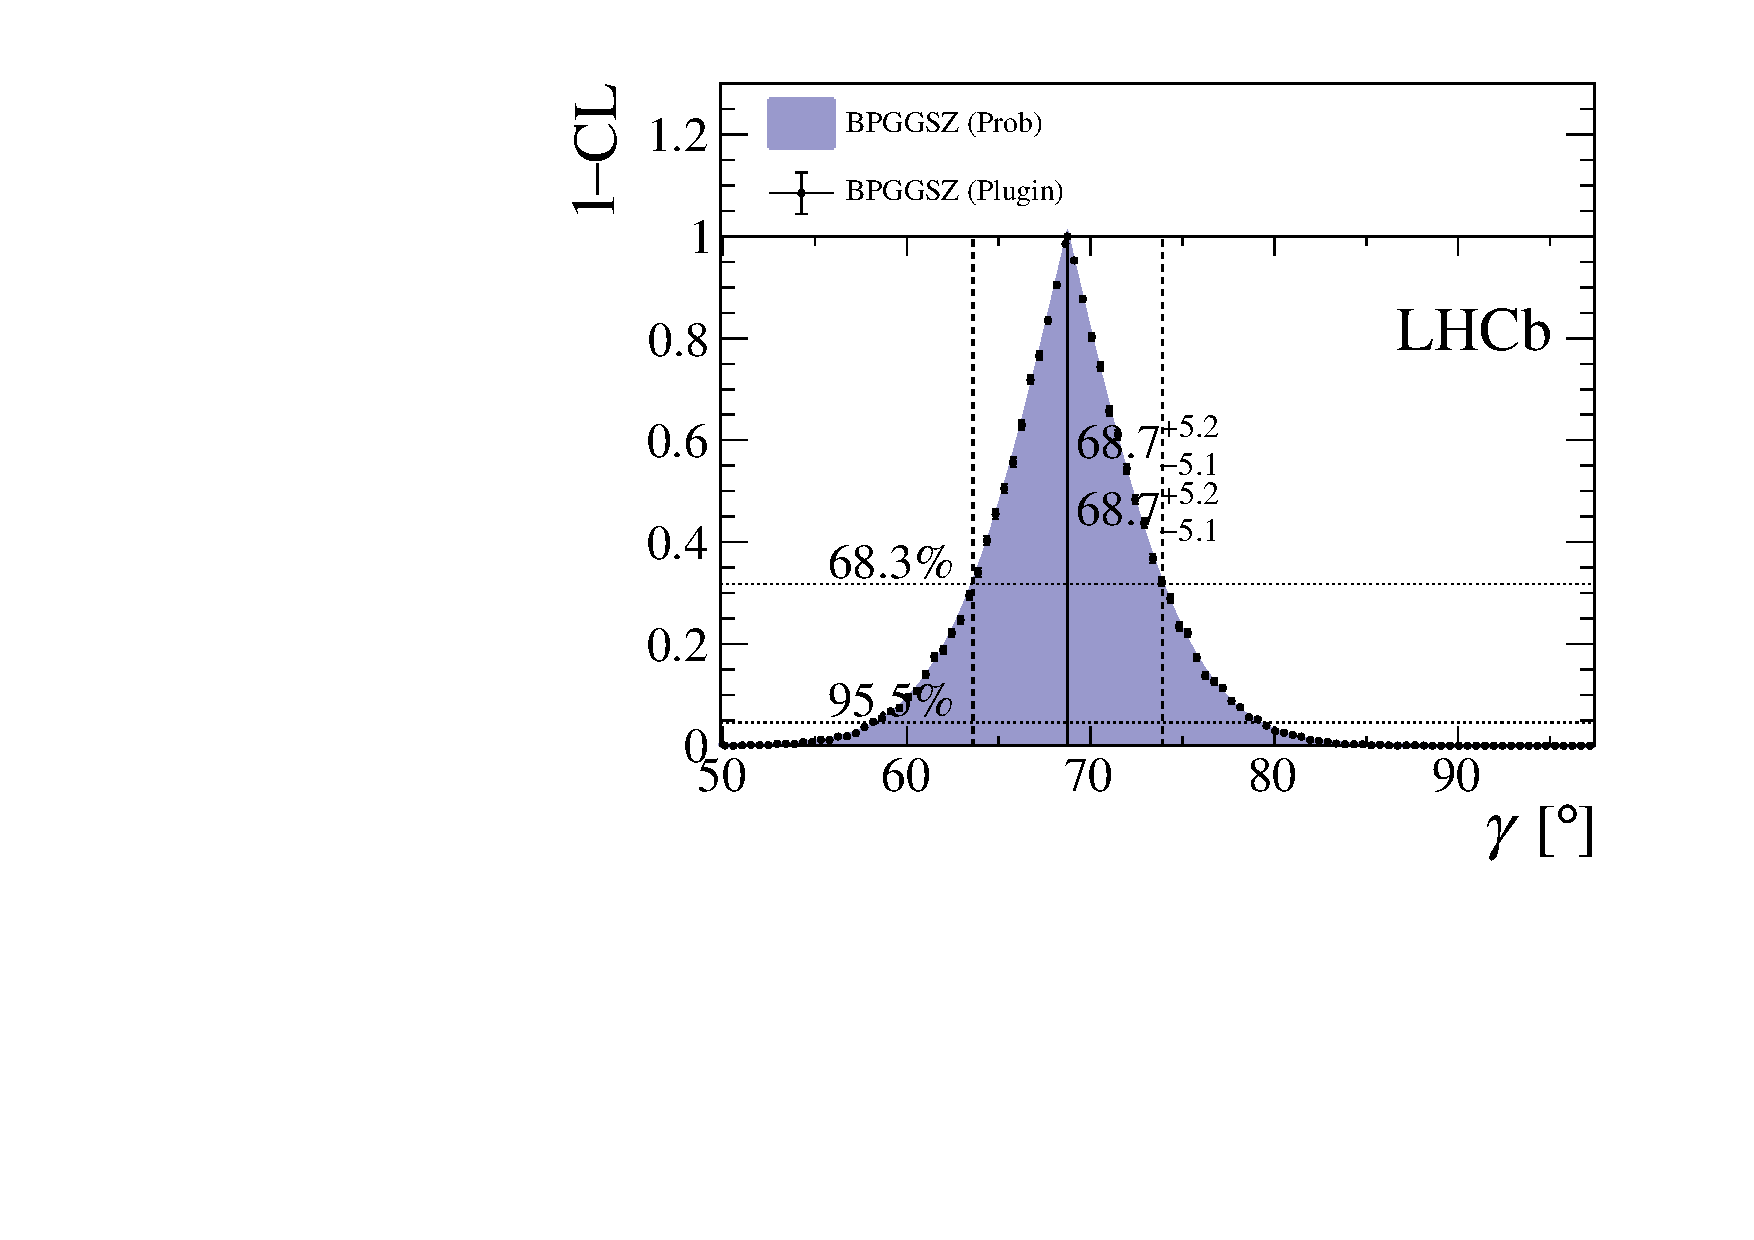
\includegraphics[width=0.75\columnwidth]{figures/analysis/interpretation/g_plugin.pdf}
    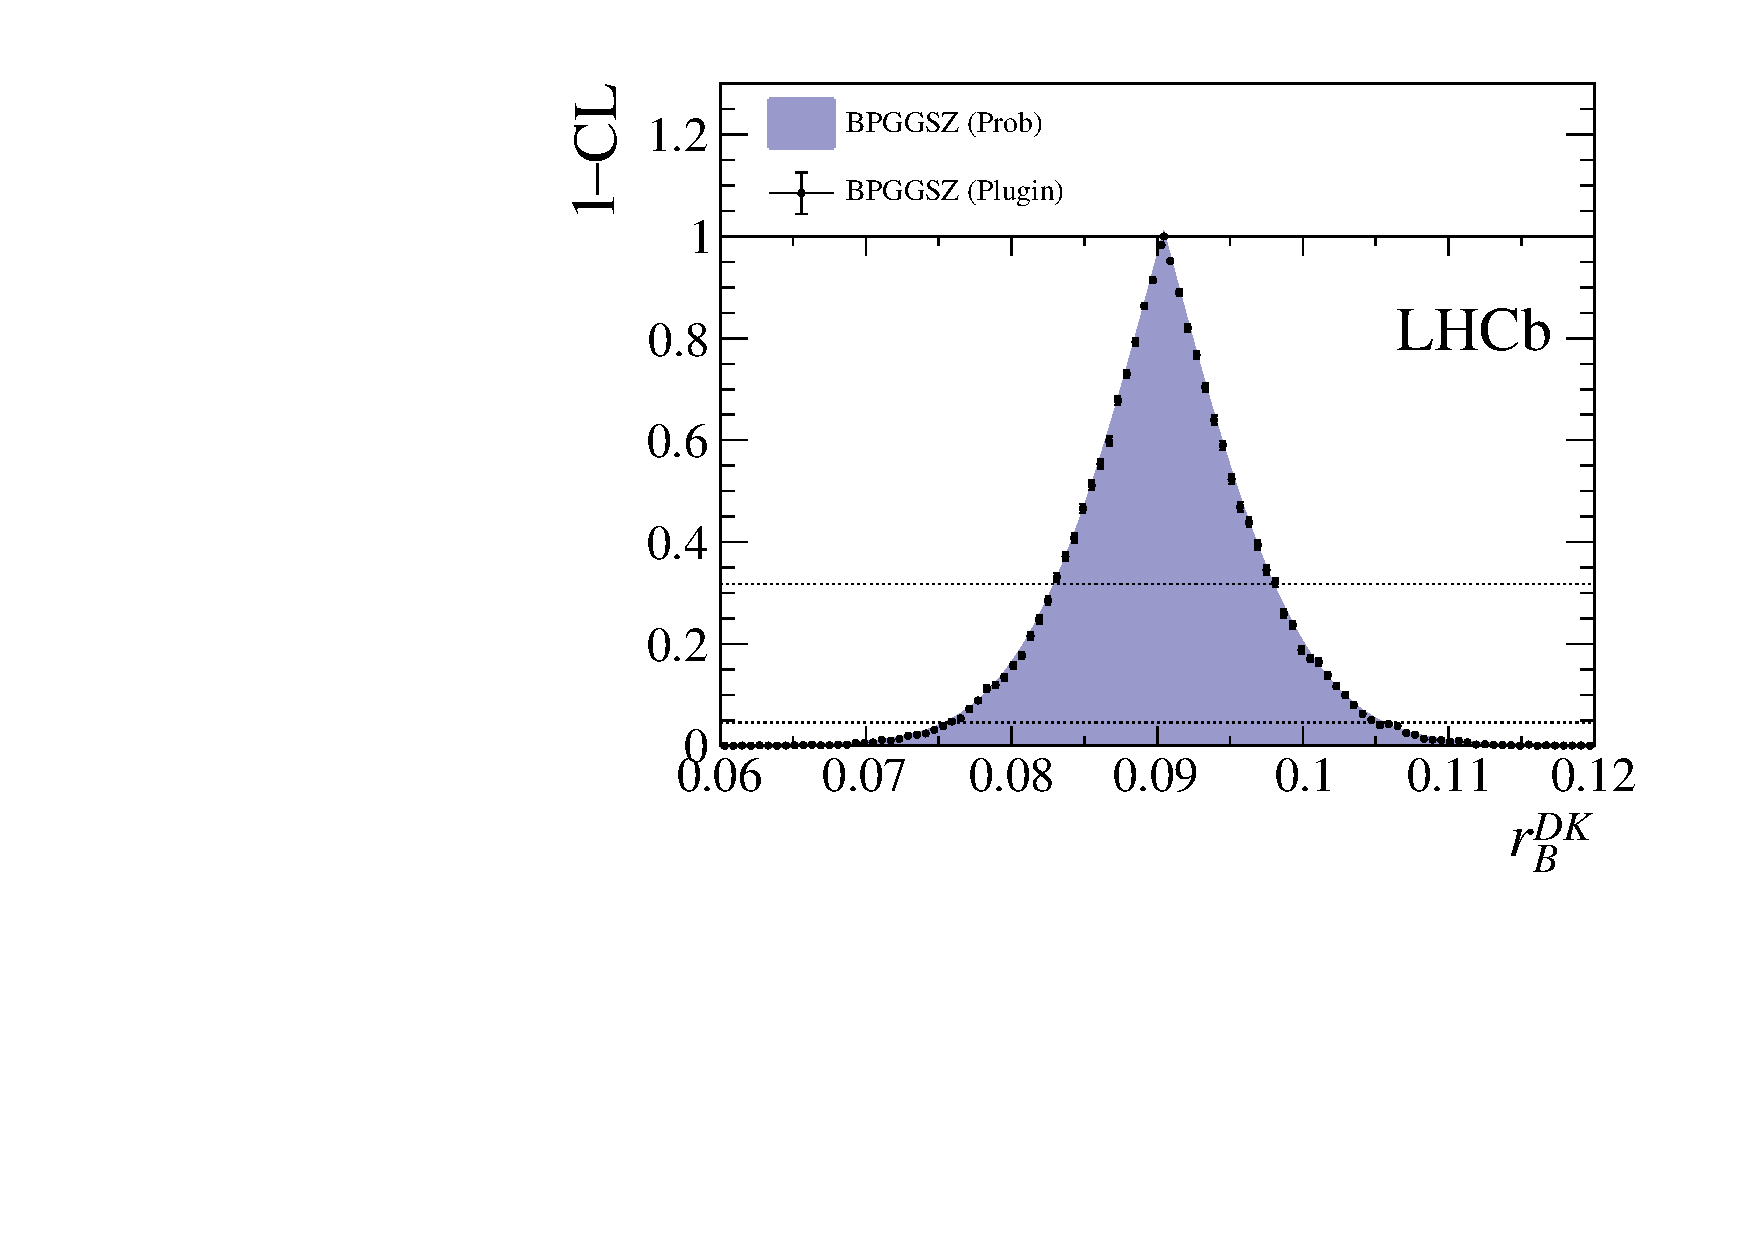
\includegraphics[width=0.45\columnwidth]{figures/analysis/interpretation/r_dk_plugin.pdf}
    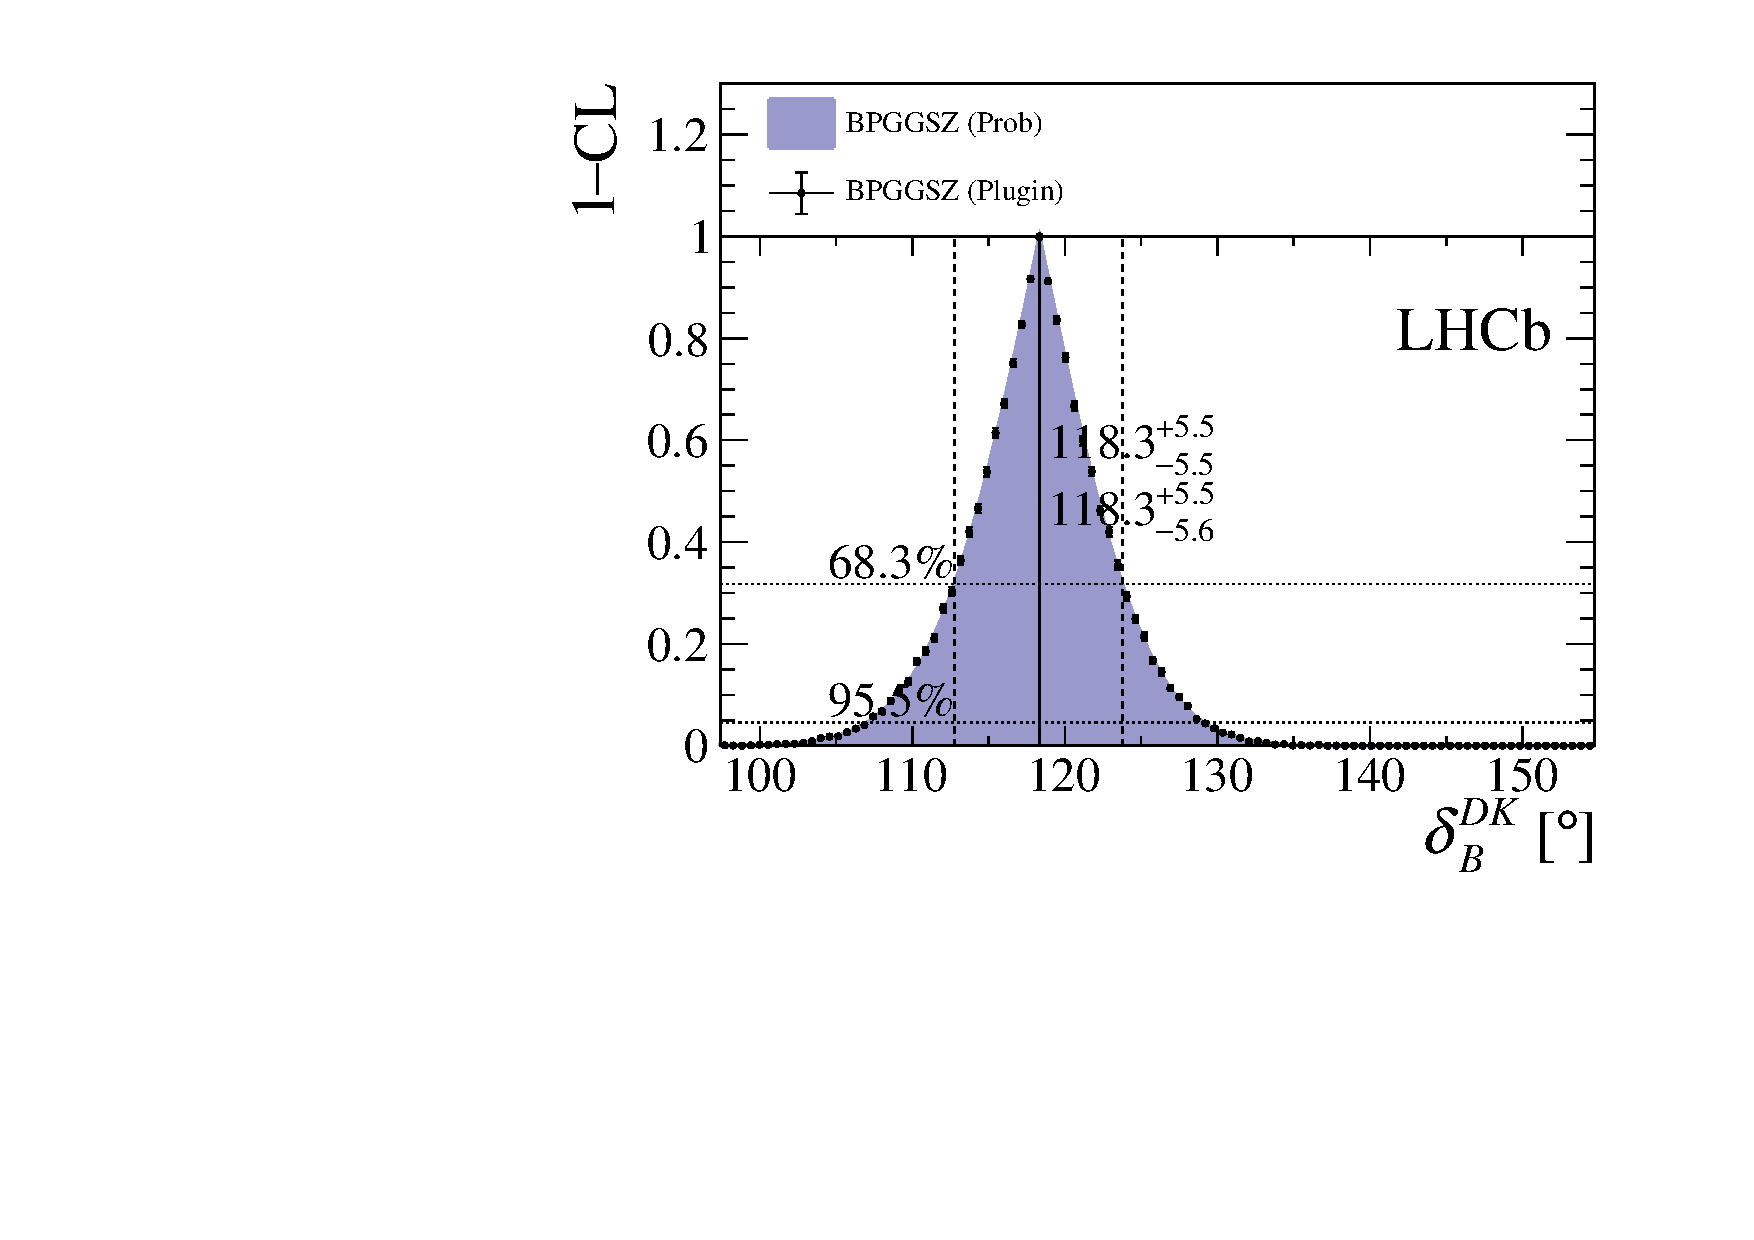
\includegraphics[width=0.45\columnwidth]{figures/analysis/interpretation/d_dk_plugin.pdf}
    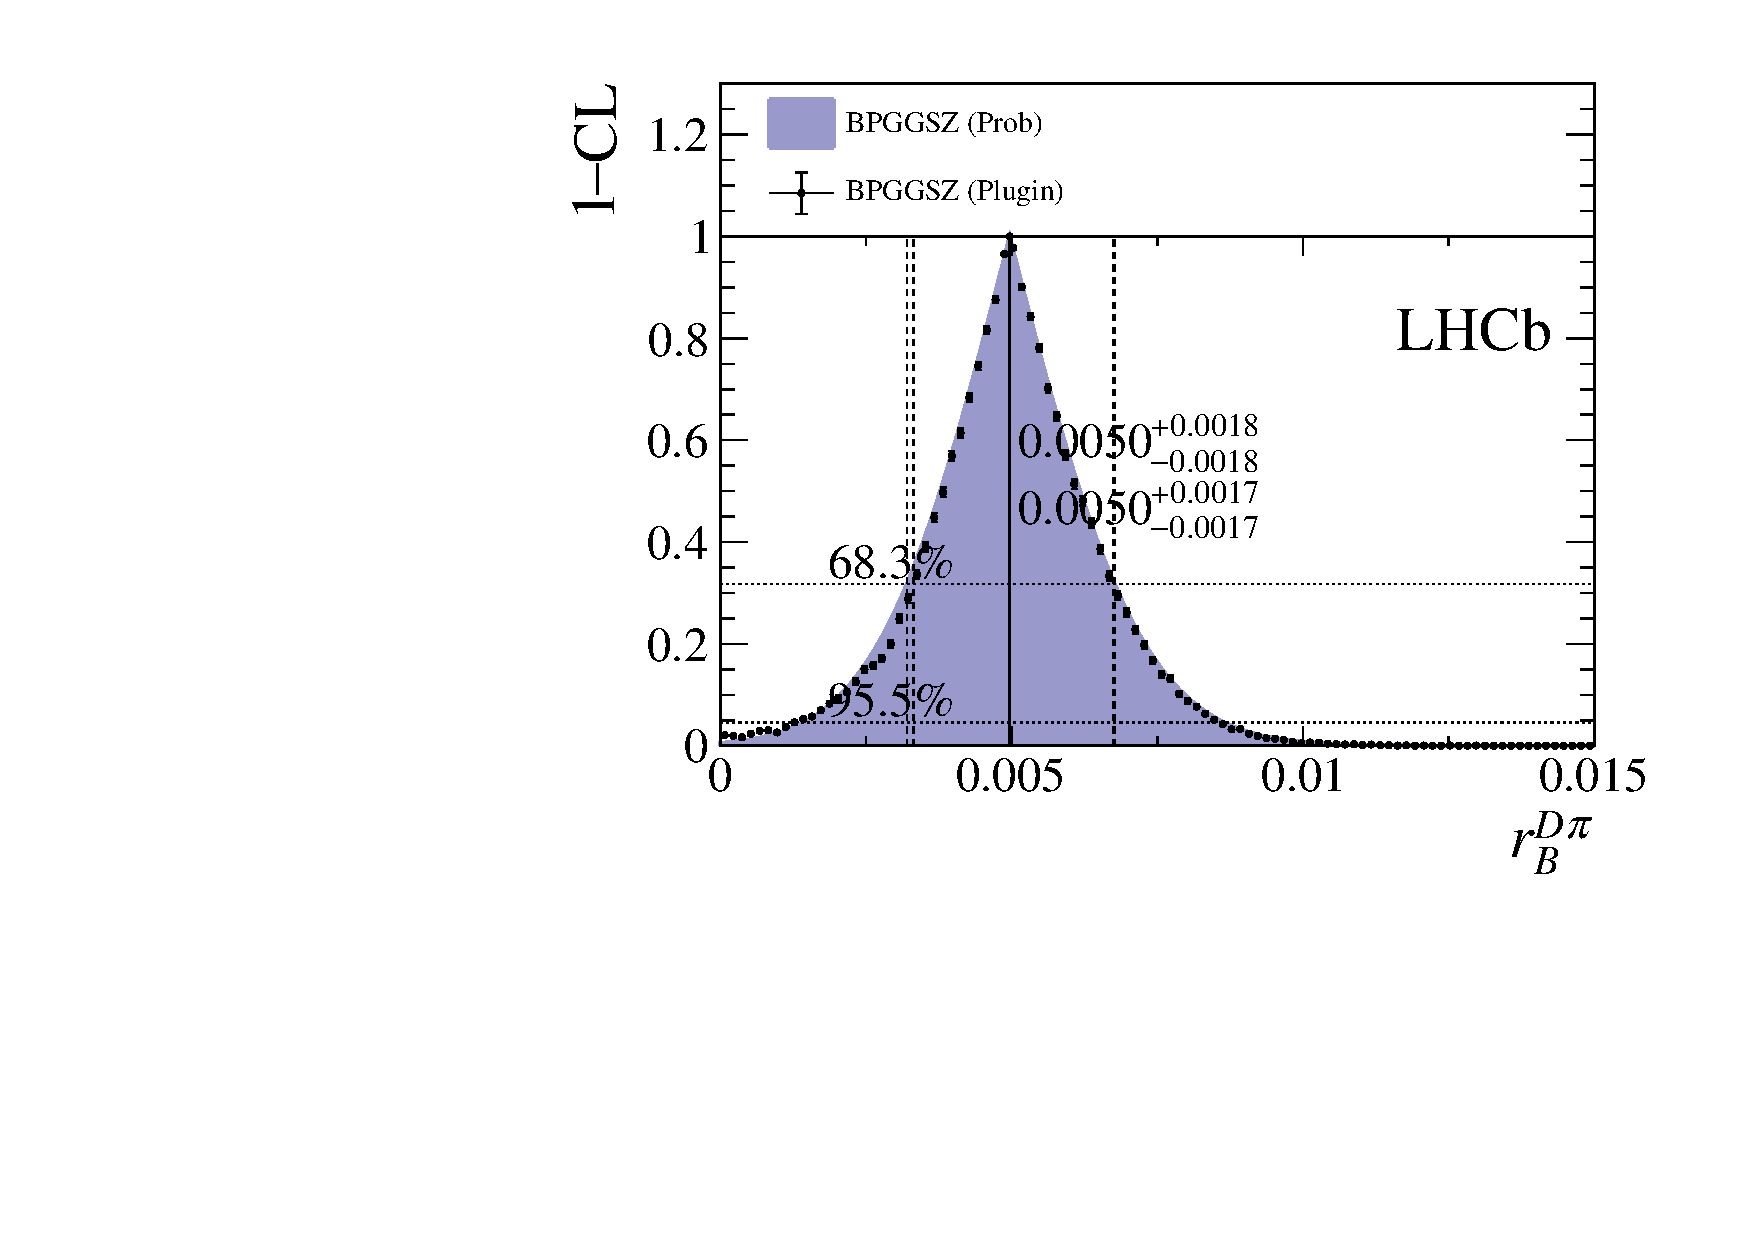
\includegraphics[width=0.45\columnwidth]{figures/analysis/interpretation/r_dpi_plugin.pdf}
    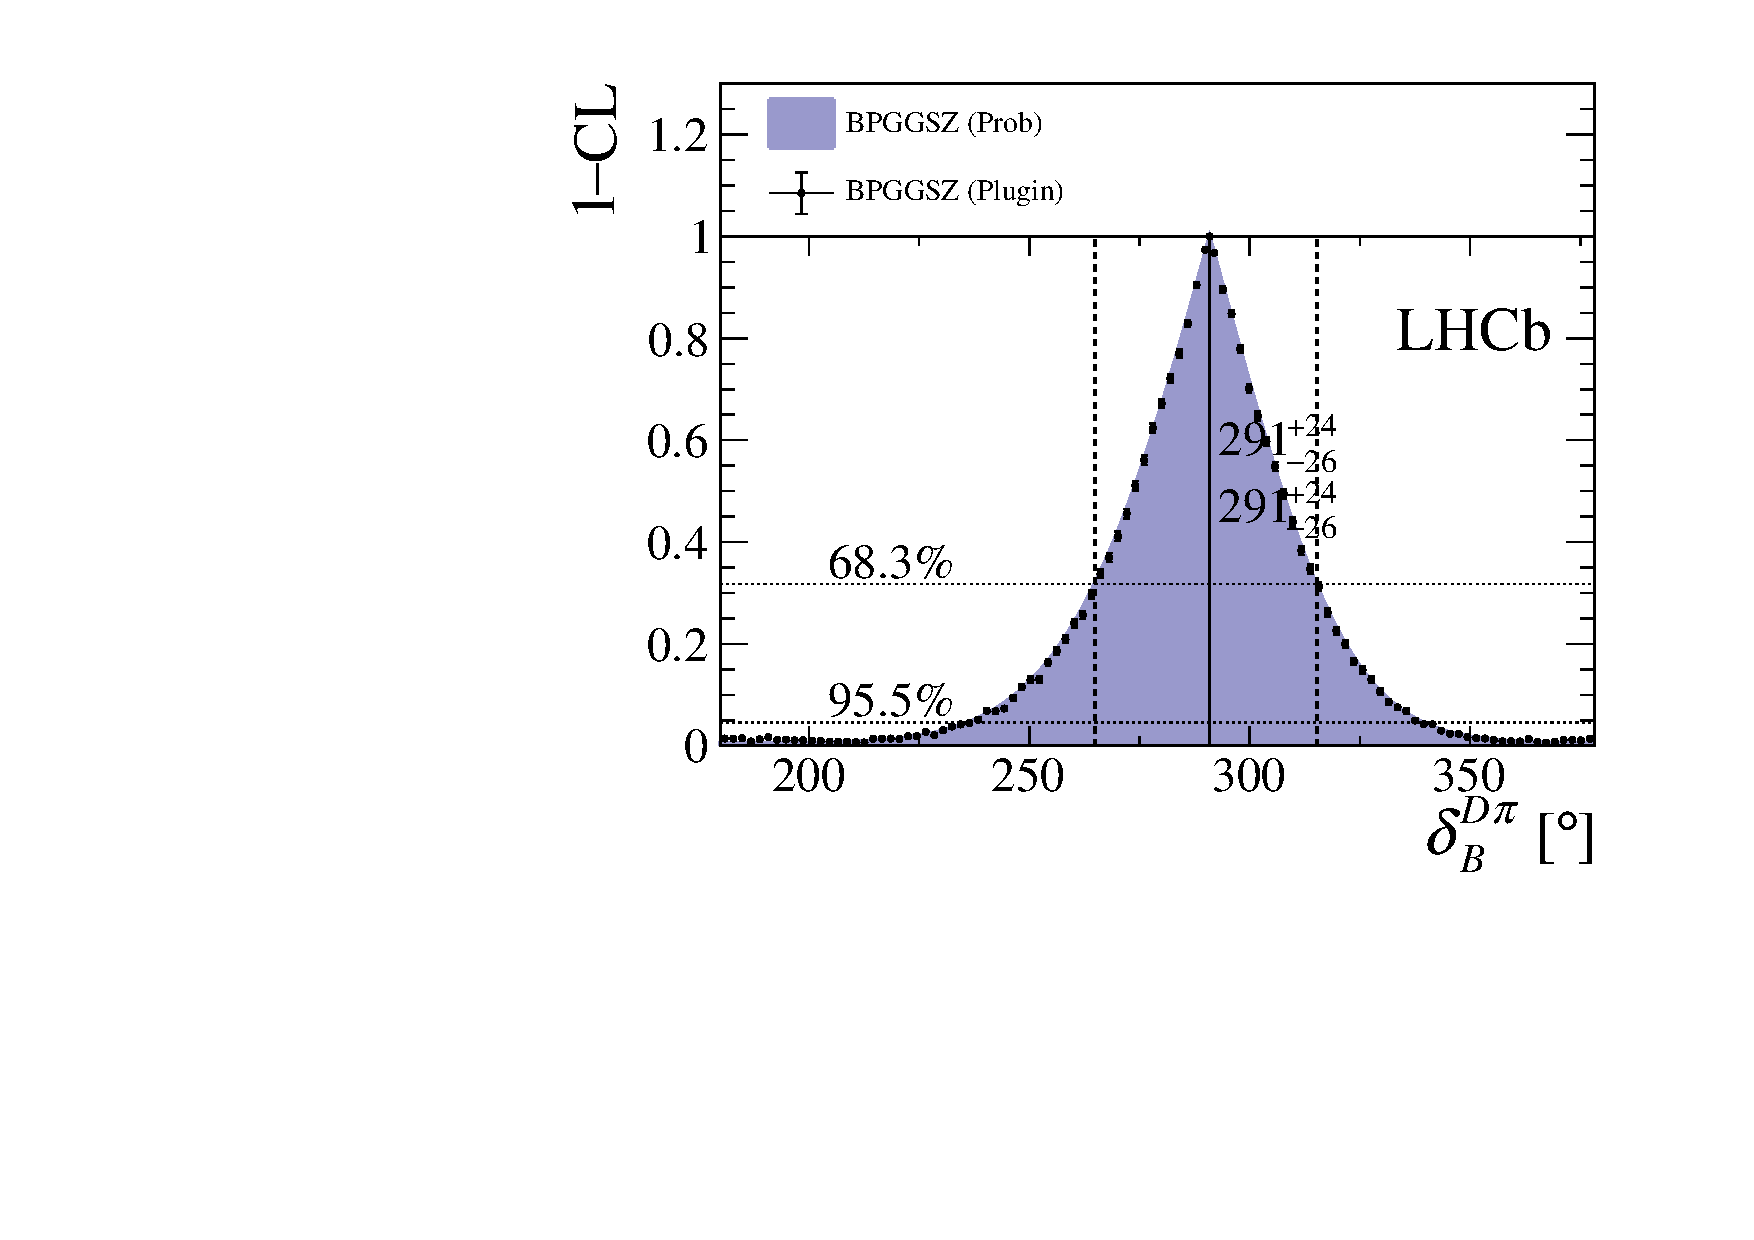
\includegraphics[width=0.45\columnwidth]{figures/analysis/interpretation/d_dpi_plugin.pdf}
    \caption{Confidence levels for the physics parameters of interest. The solutions are written on the plots, where the top number is given with \texttt{PROB} uncertainties and the bottom number with \texttt{PLUGIN} uncertainties.}
    \label{fig:1d_CL}
\end{figure}

\begin{figure}[tp]
    \centering
    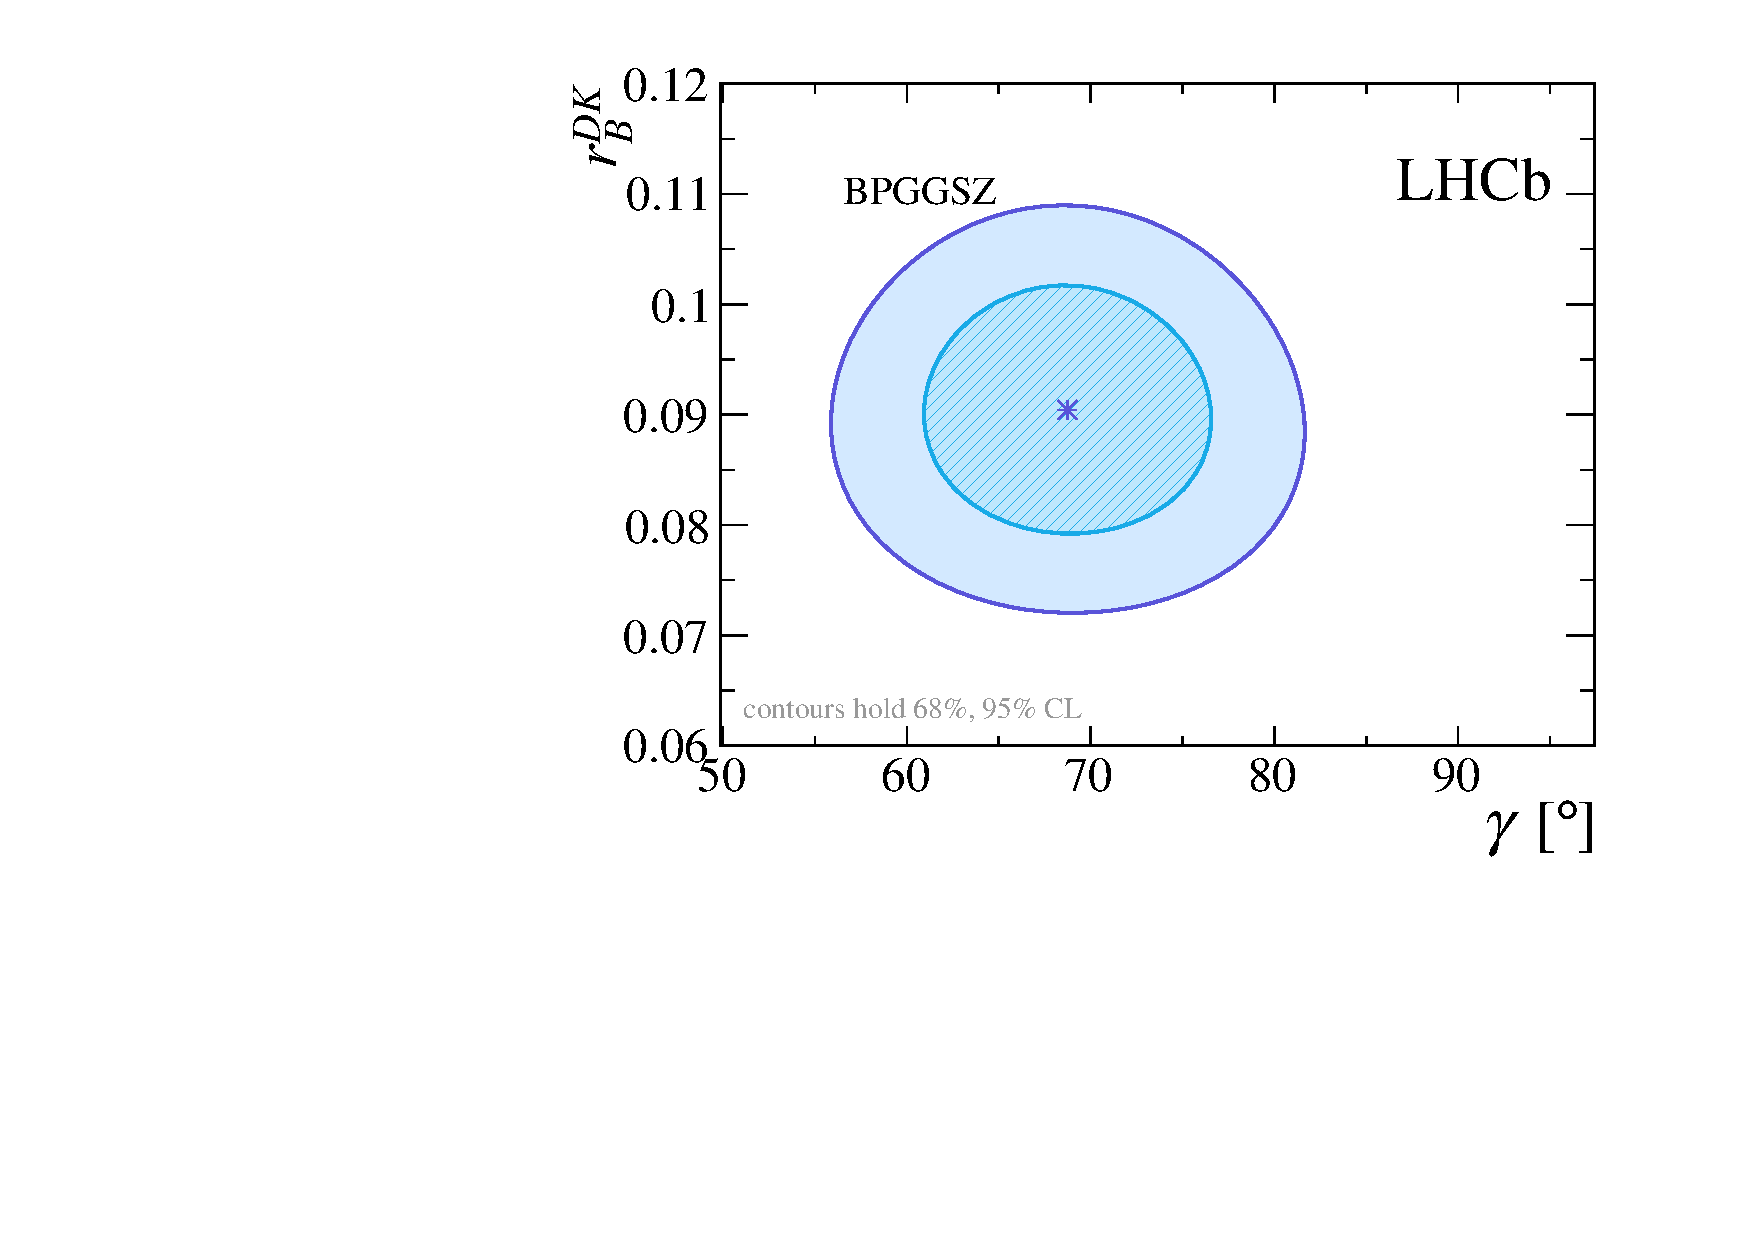
\includegraphics[width=0.41\columnwidth]{figures/analysis/interpretation/2d_g_r_dk_prob.pdf}
    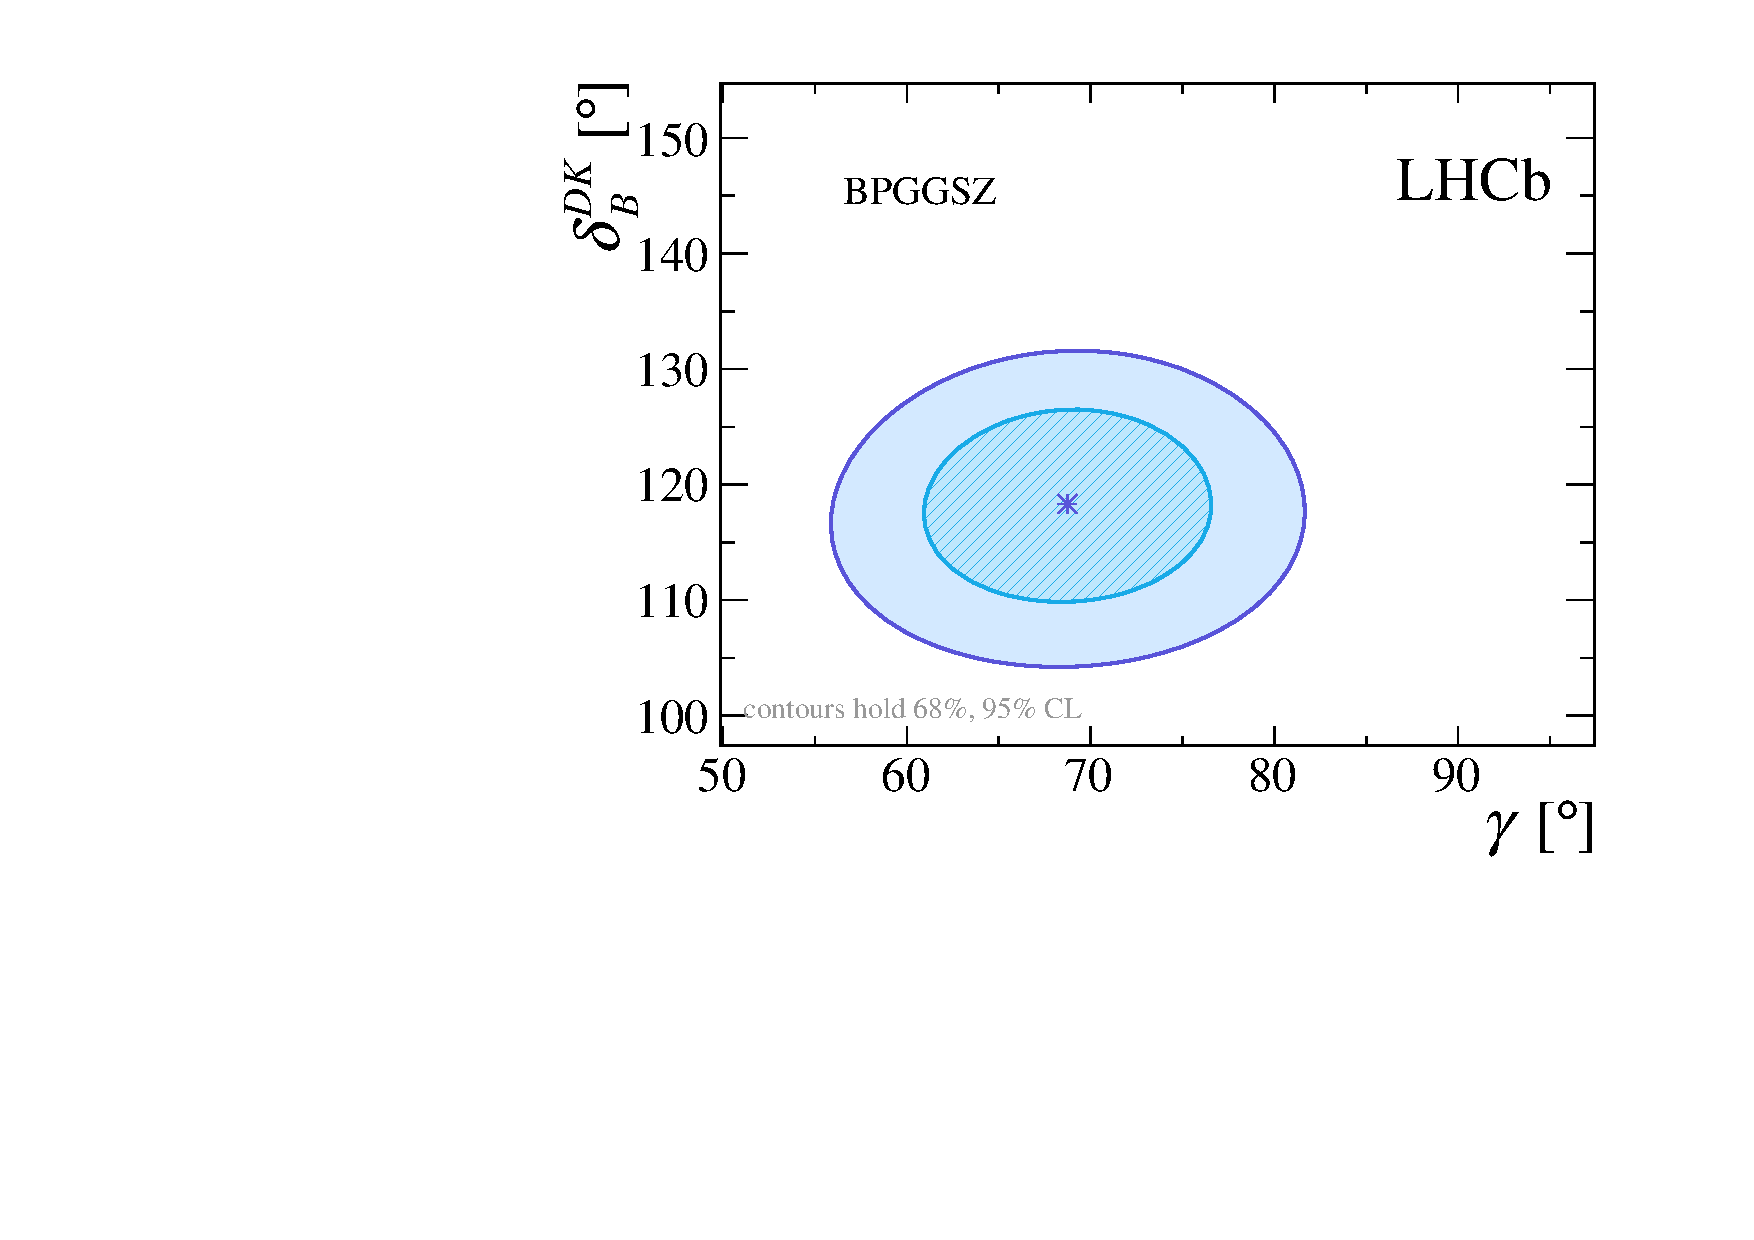
\includegraphics[width=0.41\columnwidth]{figures/analysis/interpretation/2d_g_d_dk_prob.pdf}
    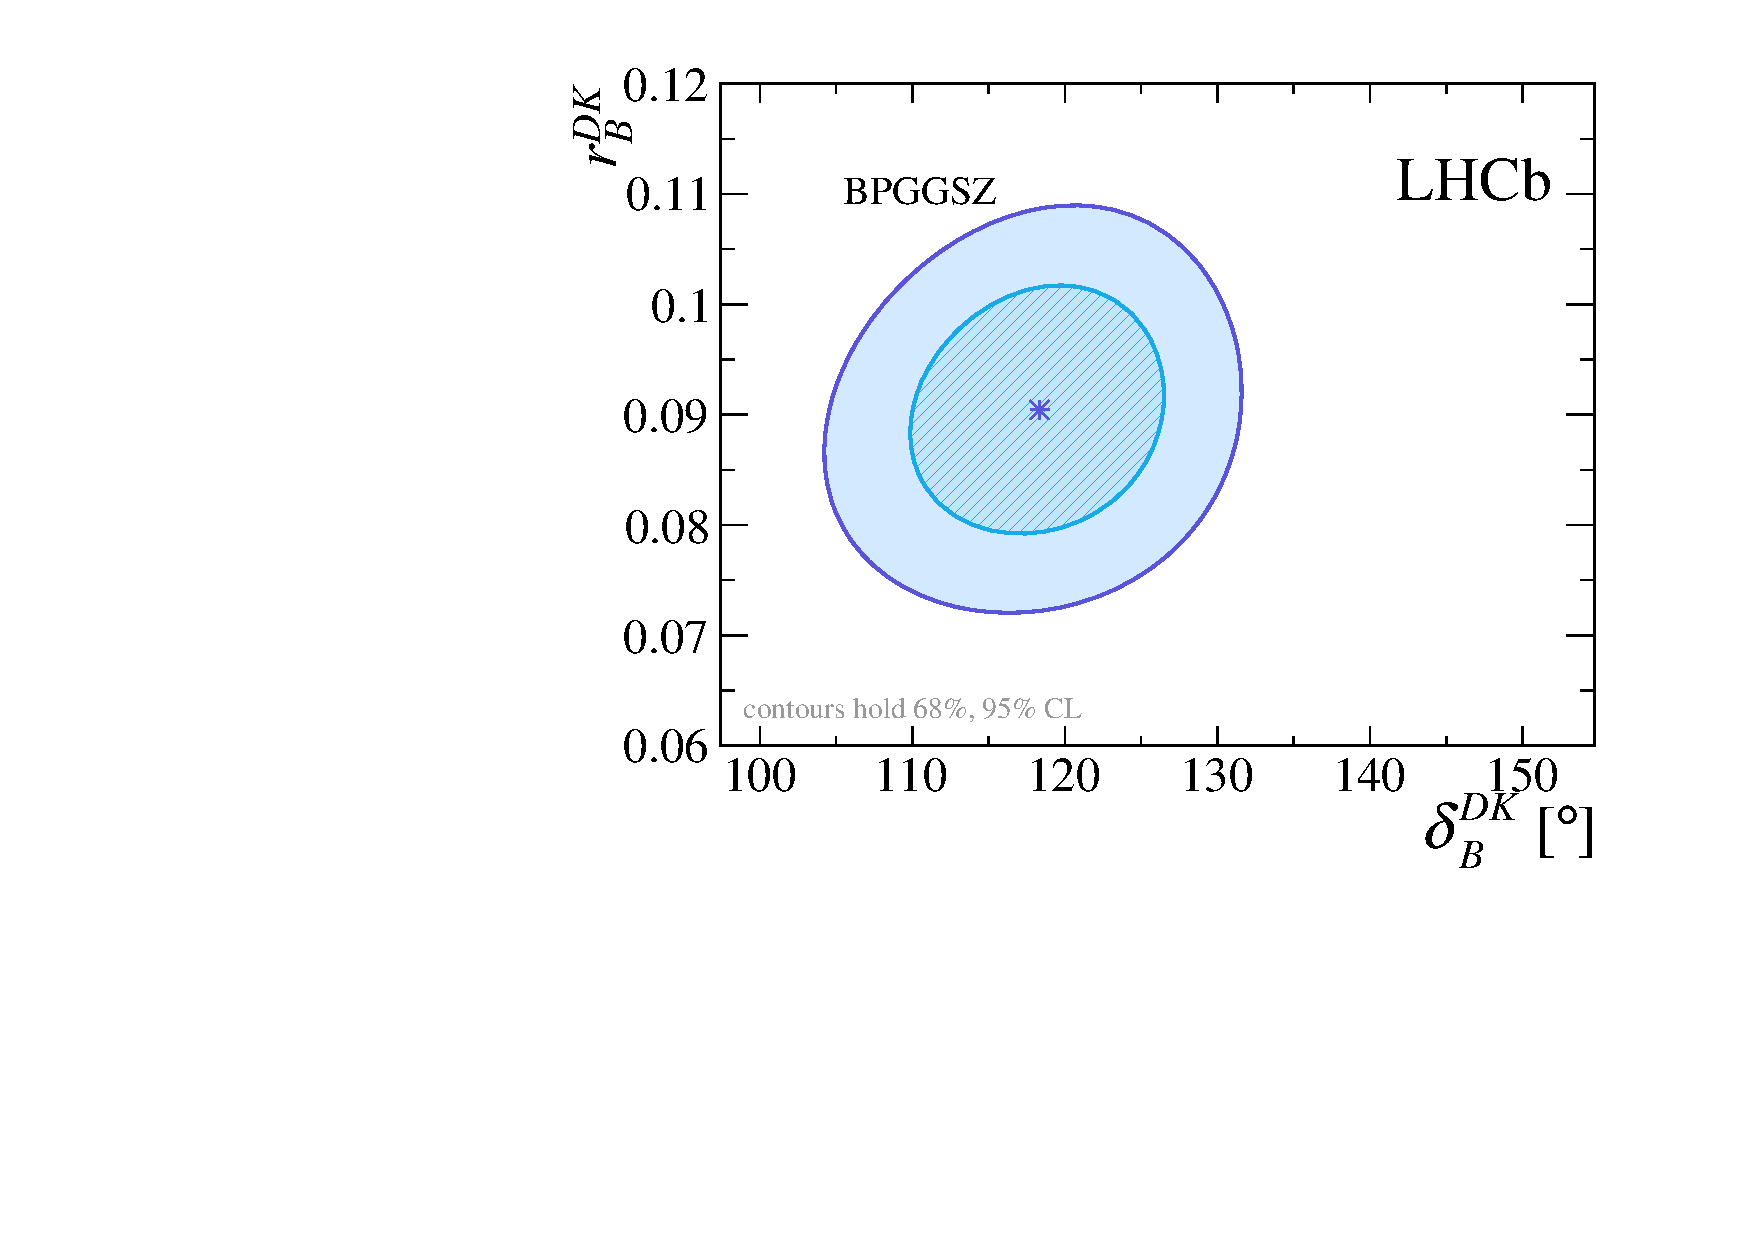
\includegraphics[width=0.41\columnwidth]{figures/analysis/interpretation/2d_d_dk_r_dk_prob.pdf}
    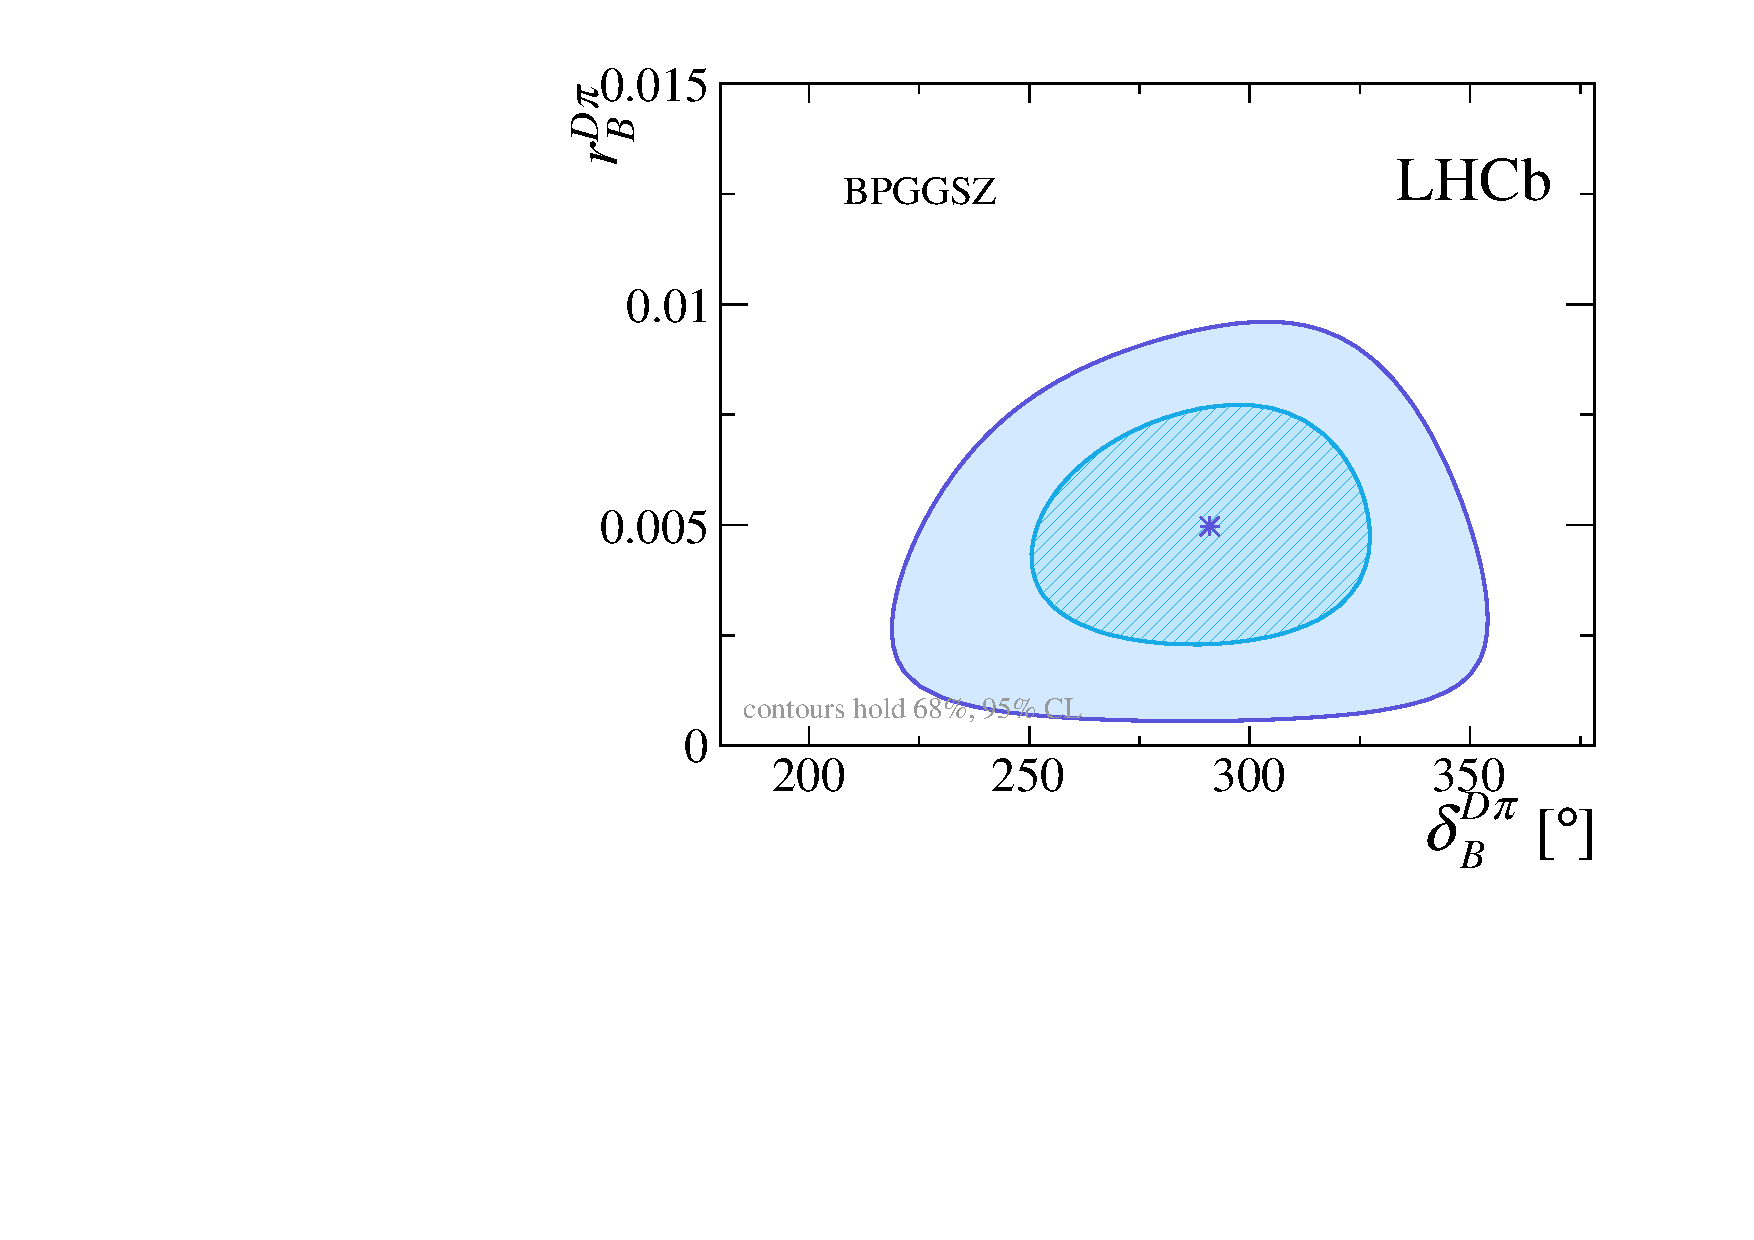
\includegraphics[width=0.41\columnwidth]{figures/analysis/interpretation/2d_d_dpi_r_dpi_prob.pdf}
    \caption{The 68\,\% and 95\,\% confidence regions for combinations of the physics parameters of interest, as obtained from the results of this measurement. The regions are calculated via the \texttt{PROB} method of \texttt{gammacombo}.}
    \label{fig:2d_CL}
\end{figure}



The contribution to the uncertainty on $\gamma$ from each of the statistical, strong-phase-related, and \lhcb-related uncertainties in isolation can be estimated by repeating the interpretation while only including subsets of the uncertainties on the input parameters. Such studies have been performed using the \texttt{PROB} method. Running with statistical uncertainties only yields an uncertainty on $\gamma$ of $5.05^\circ$. Including only the statistical and \lhcb-related systematic uncertainties yields an uncertainty on $\gamma$ of $5.08^\circ$, suggesting that the \lhcb-related systematics  contribute an uncertainty of $0.6^\circ$. This is a reduction compared to earlier analyses, where the contribution was about $2^\circ$. A significant contribution to the improvement is the efficiency-related systematic that has been avoided by promoting $\BtoDpi$ to a signal channel. Including only the statistical and the strong-phase-related uncertainties leads to an uncertainty on $\gamma$ of $5.09^\circ$, showing the strong-phase-related uncertainty to be $0.6^\circ$, somewhat lower than the expectation of $1.2^\circ$  presented in Ref.~\cite{BESCISI}. This is partly because the uncertainty estimate of that paper does not take into account the use of the \DtoKsKK channel, and partly because the uncertainty estimate depends on the specific central values.

The obtained statistical uncertainty on $\gamma$ is in excellent agreement with the expectation from pseudoexperiments. The interpretation procedure outlined above has been performed for each of the pseudoeexperiments performed to establish the feasibility of the \CP fit in Section~\ref{sub:fit_setup} (including only statistical uncertainties on the observables) and the central 90\,\% interval of the obtained uncertainties is $[4.4^\circ, 6.0^\circ]$. Similar studies have been carried out where no background decays are included in the generated toy data sets. In this case, the precision on $\gamma$ is improved by about 30\,\%.

\subsection{Compatibility with other measurements} % (fold)
\label{sub:compatibility_with_other_measurements}

It is worth comparing the obtained constraints on the physics parameters with the information available from other measurements, made at the \B factories and by the \lhcb collaboration using other decay channels. This comparison is made for $\gamma$ and the hadronic parameters in the \BtoDK decay in Fig.~\ref{fig:all_gamma_results}, comparing to the results of the combinations of $\gamma$ measurements by the Belle~\cite{BelleCombo} and BaBar~\cite{BabarCombo} collaborations presented in 2013, and the 2018 combination of \lhcb results~\cite{LHCb-CONF-2018-002}. For this purpose, the \lhcb combination is re-performed,  removing the input from earlier BPGGSZ measurements that use \BtoDK decays, because they were made using data that is re-analysed in the present thesis; thus they need to be excluded to make the results that are compared independent. The combination employs the same statistical method outlined above, with the exception that the likelihood now depends on observables measured in a number of different analyses. The included measurements are summarised in Table~\ref{tab:inputs}. It can be seen in Fig.~\ref{fig:all_gamma_results} that the results obtained in this thesis agree well with the Belle and BaBar results, but are in some tension with the 2018 \lhcb combination, especially for the $\delta_B^{DK}$ parameter.

\begin{figure}[tb]
    \centering
    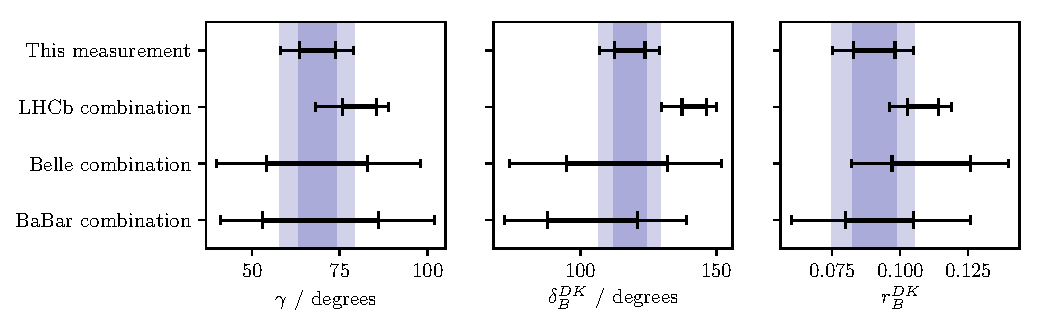
\includegraphics[width=\columnwidth]{figures/analysis/interpretation/experiment_comparison.pdf}
    \caption{Comparison of the $1\sigma$ and $2\sigma$ confidence intervales obtained results for $\gamma$ and the physics parameters relating to \BtoDK decays, with those from the combinations of $\gamma$ measurements by the Belle~\cite{BelleCombo} and BaBar~\cite{BabarCombo} collaborations, and the 2018 combination of \lhcb results~\cite{LHCb-CONF-2018-002} where the BPGGSZ measurements have been excluded.}
    \label{fig:all_gamma_results}
\end{figure}

The level of compatibility can be quantified by calculating the three-dimensional $\chi^2$ of the BPGGSZ results and those of the \lhcb combination (without the earlier BPGGSZ measurements), with respect to the best fit values of $(\gamma, r_B^{\DK}, \delta_B^{\DK})$ when all measurements are combined. The two-dimensional confidence regions obtained in these three cases are compared in Fig.~\ref{fig:lhcb_dk_comp_2d}, where some tension in $r_B^{\DK}$ and $\delta_B^{\DK}$ is visible again. The calculation is based on the \texttt{PLUGIN} uncertainties; for the \lhcb combination these uncertainty estimates are slightly larger than the ones obtained via the \texttt{PROB} method. One obtains $\chi^2=\chi^2_{GGSZ}+\chi^2_\text{LHCb} = 0.7 + 9.1 = 9.8$, which for 3 degrees of freedom correspond to a $p$-value of $2\,\%$, or a $2.3\sigma$ deviation. However, this tension is expected to be reduced when other measurements in the \lhcb combination are updated to include results based on the full Run~1~and~2 data set. The most important update is that of the two-body ADS/GLW measurement in \BtoDK decays because that measurement, and the BPGGSZ measurement presented in this thesis, have the largest impact in the combination.


\begin{figure}[tp]
    \centering
    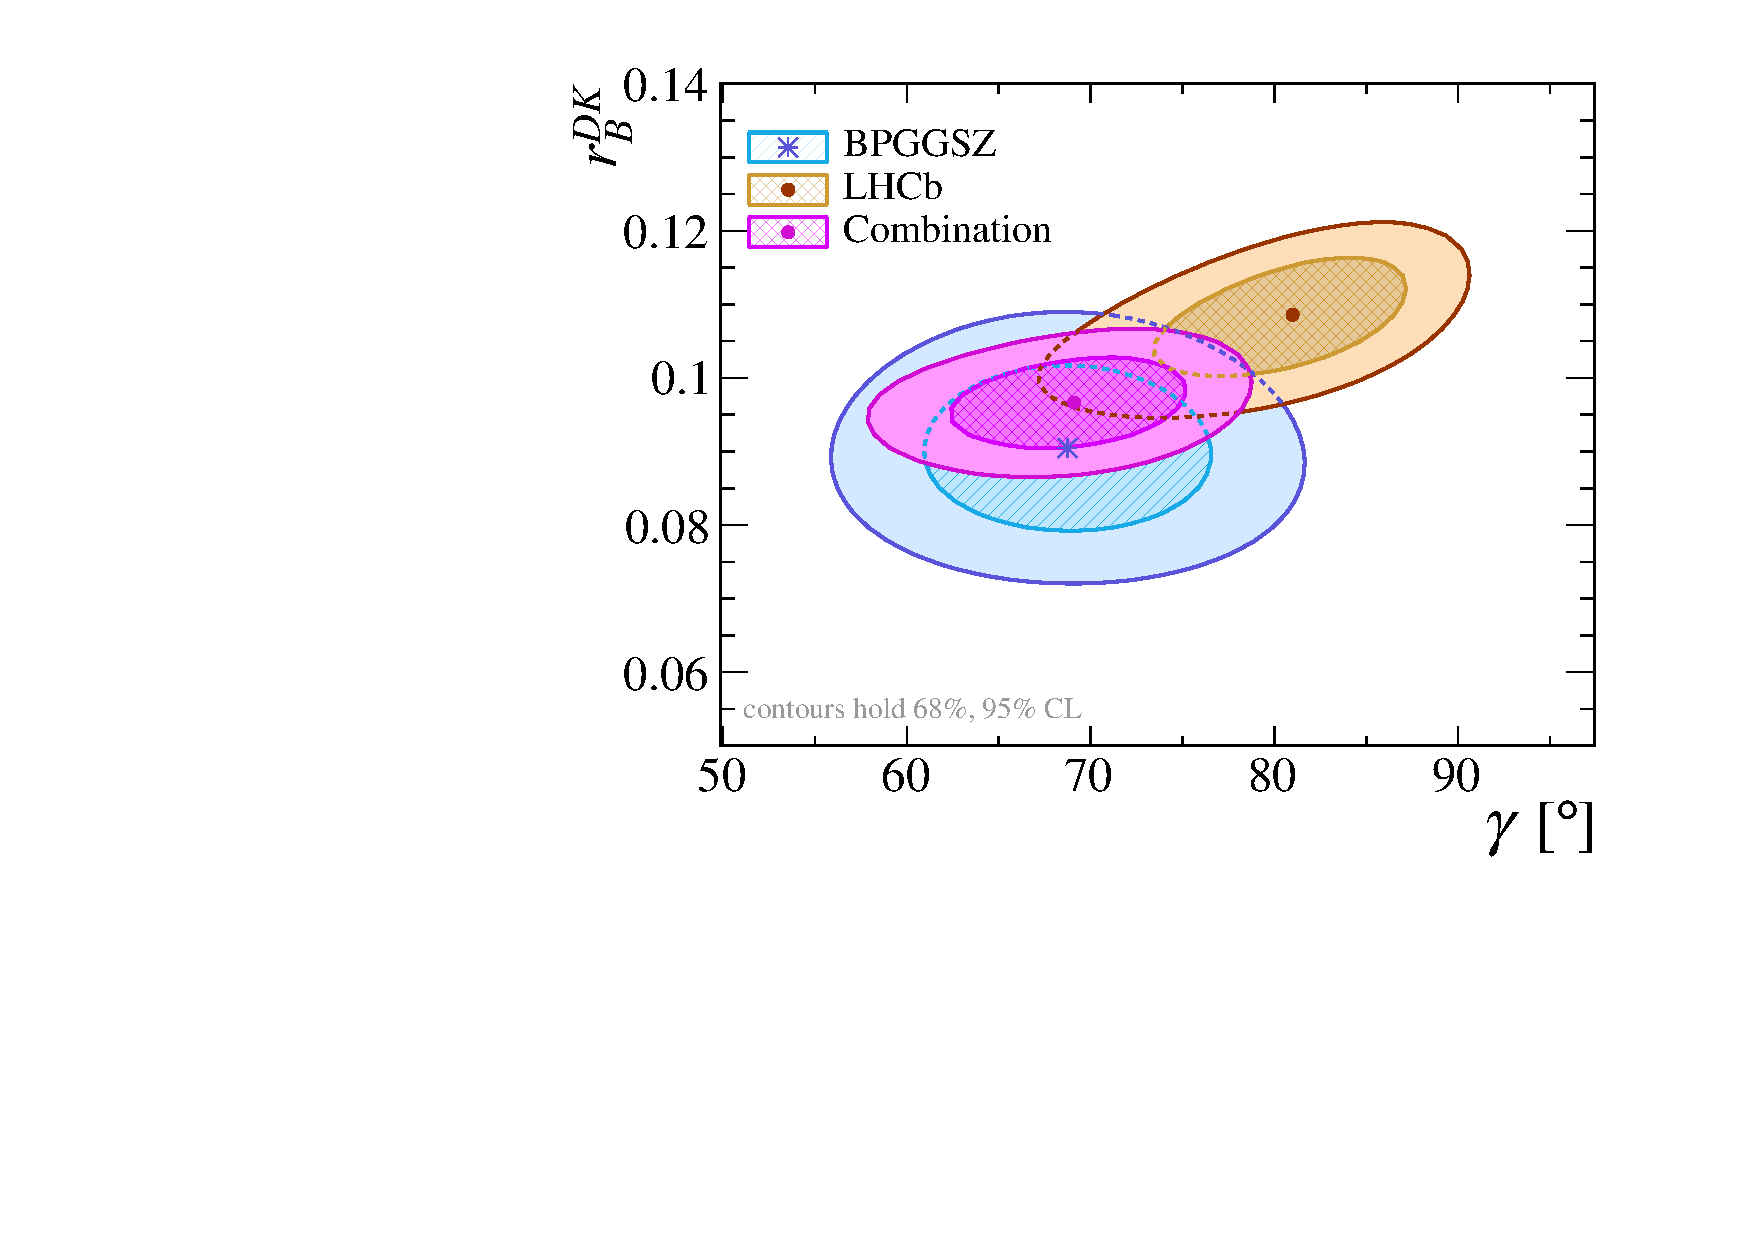
\includegraphics[width=0.45\columnwidth]{figures/analysis/interpretation/2d_g_r_dk_vs_old_lhcb_prob.pdf}
    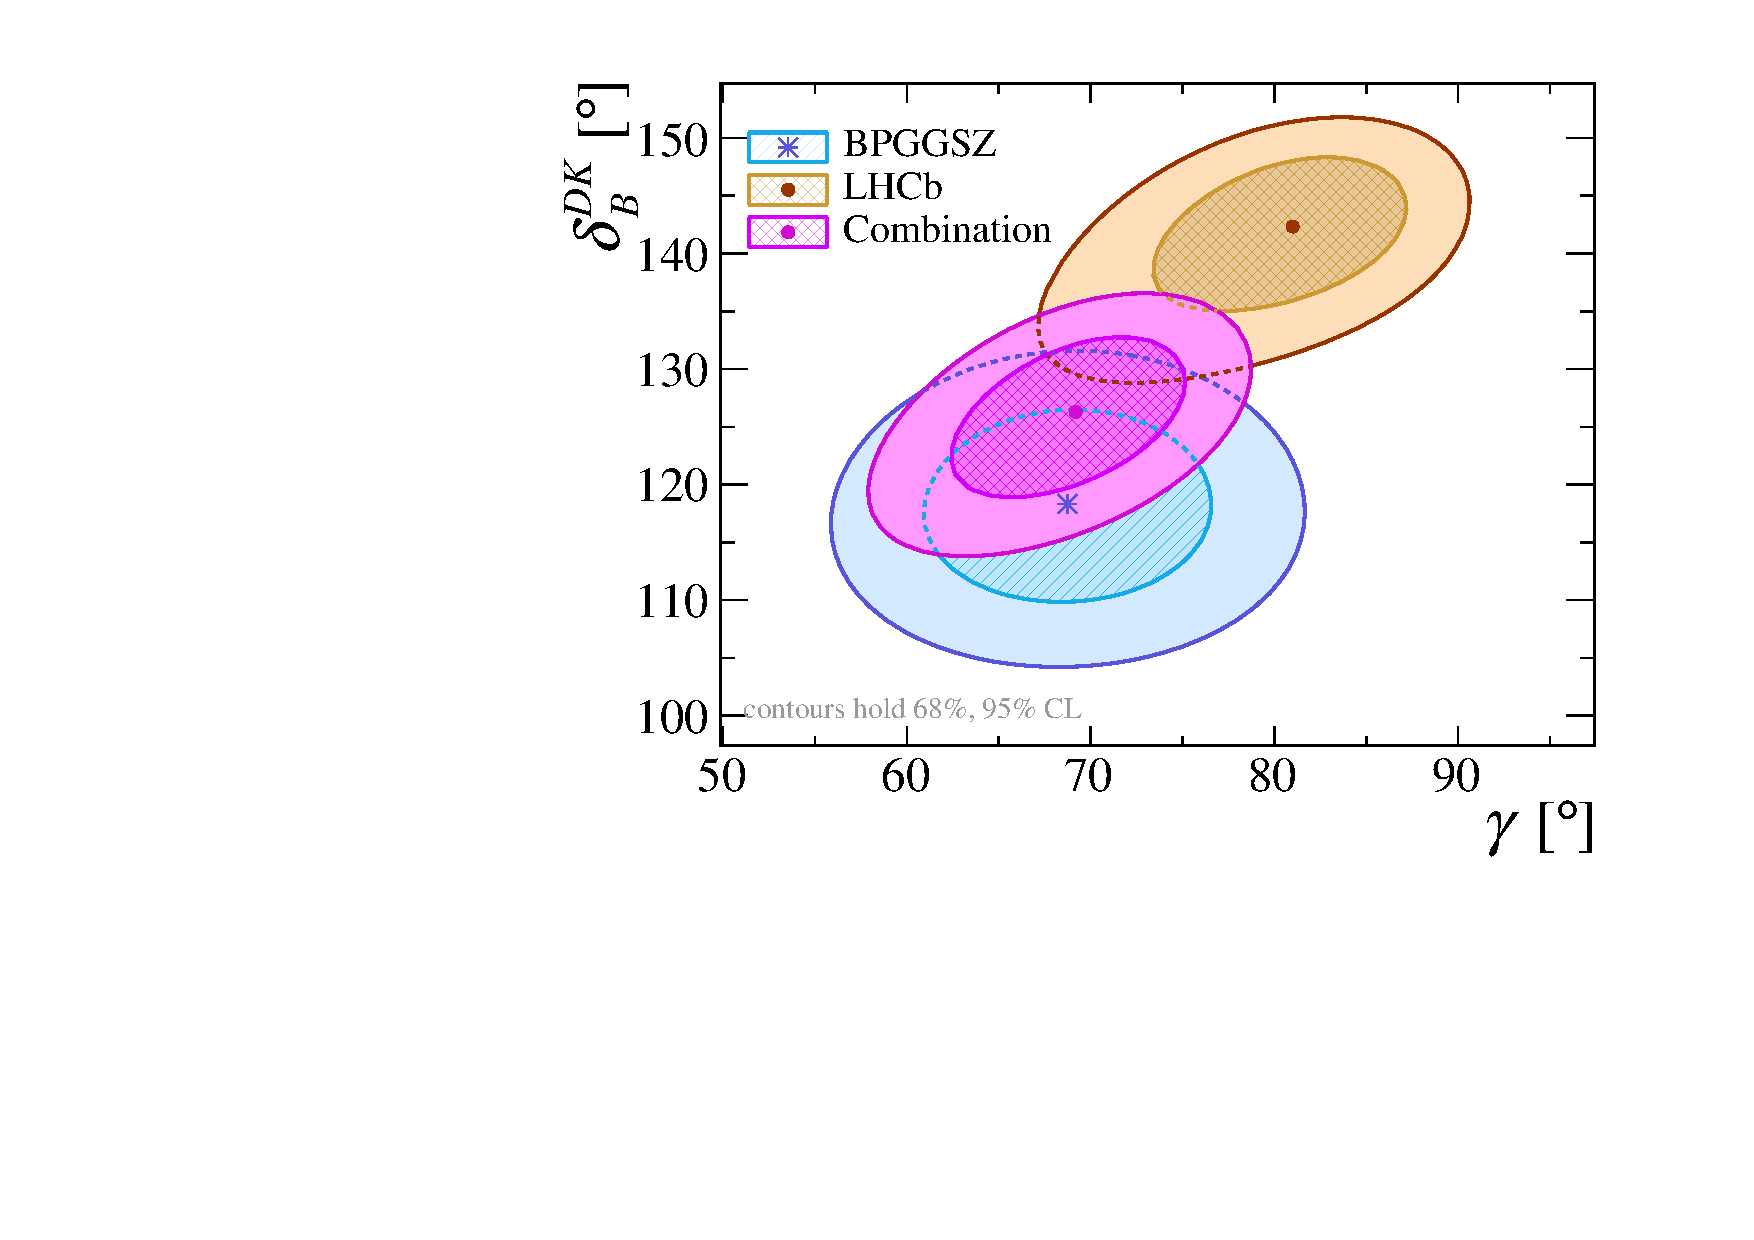
\includegraphics[width=0.45\columnwidth]{figures/analysis/interpretation/2d_g_d_dk_vs_old_lhcb_prob.pdf}
    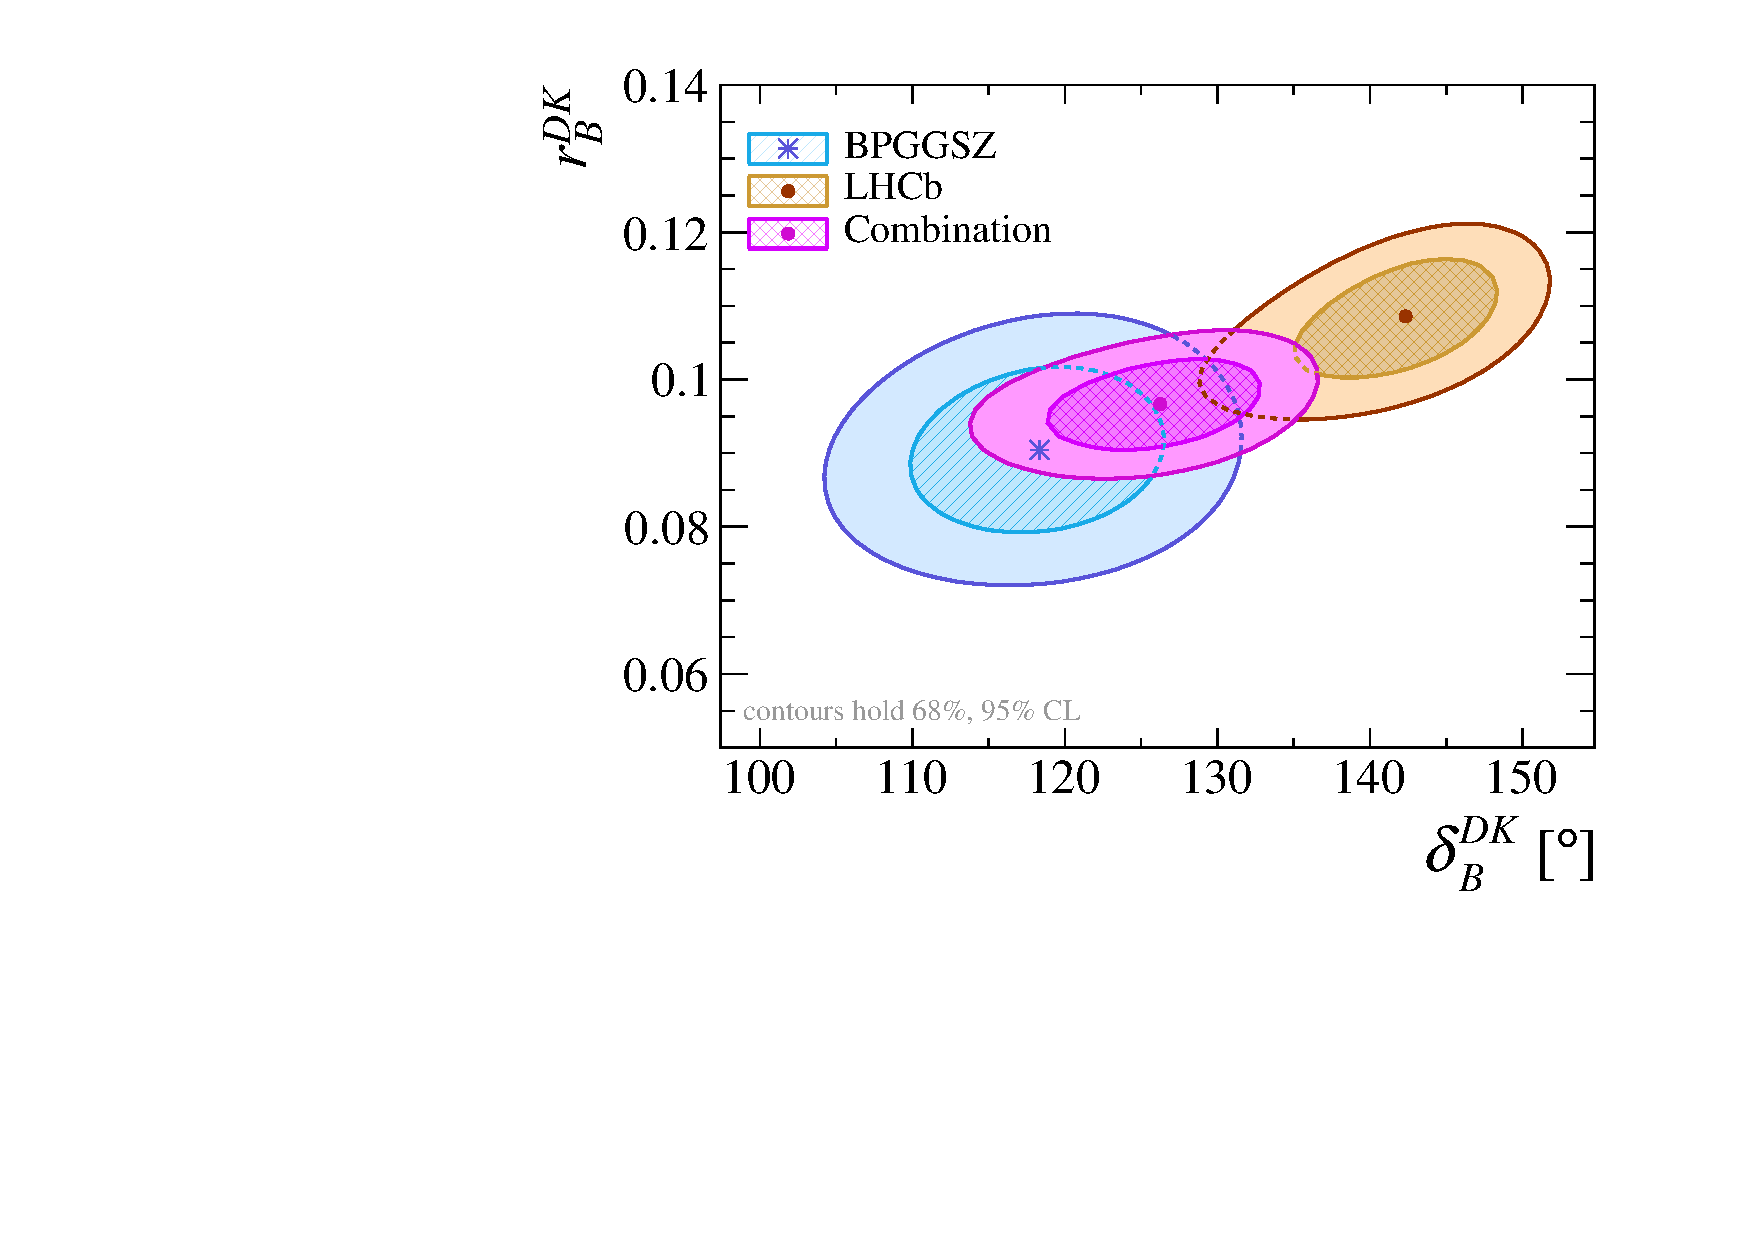
\includegraphics[width=0.45\columnwidth]{figures/analysis/interpretation/2d_d_dk_r_dk_vs_old_lhcb_prob.pdf}
    \caption{The 68\,\% and 95\,\% confidence regions  for $(\gamma, r_B^{\DK})$, $(\gamma, \delta_B^{\DK})$, and $(\delta_B^{\DK}, r_B^{\DK})$ for this measurement, the 2018 \lhcb combination~\cite{LHCb-CONF-2018-002} where the BPGGSZ results have been excluded, and the combination thereof, calculated via the \texttt{PROB} method of \texttt{gammacombo}.}
    \label{fig:lhcb_dk_comp_2d}
\end{figure}

\begin{table}[tp]
  \caption{List of the LHCb measurements used in the combination that the results obtained in the present thesis is compared to. These correspond to the 2018 \lhcb combination~\cite{LHCb-CONF-2018-002}, except that the earlier BPGGSZ results made with \BtoDK decays have not been included in the comparison. In the method column, TD stands for "time-dependent".}
  \begin{center}
      \renewcommand{\arraystretch}{1.25}
      \begin{tabular}{l l l l l }
        \toprule
        $\B$ decay  & $\D$ decay & Method   & Ref. & Data set   \\
        \midrule
        \BuDK     & \Dhh      & GLW         & \cite{LHCb-PAPER-2017-021} & 2011-16  \\
        \BuDK     & \Dhh      & ADS         & \cite{LHCb-PAPER-2016-003} & 2011-12       \\
        \BuDK     & \Dhpipipi & GLW/ADS     & \cite{LHCb-PAPER-2016-003} & 2011-12       \\
        \BuDK     & \Dhhpiz   & GLW/ADS     & \cite{LHCb-PAPER-2015-014} & 2011-12       \\
        \BuDK     & \DKSKpi   & GLS         & \cite{LHCb-PAPER-2013-068} & 2011-12       \\
        \BuDstK   & \Dhh      & GLW         & \cite{LHCb-PAPER-2017-021} & 2011-16  \\
        \BuDKst   & \Dhh      & GLW/ADS     & \cite{LHCb-PAPER-2017-030} & 2011-16  \\
        \BuDKst   & \Dhpipipi & GLW/ADS     & \cite{LHCb-PAPER-2017-030} & 2011-16  \\
        \BuDKpipi & \Dhh      & GLW/ADS     & \cite{LHCb-PAPER-2015-020} & 2011-12       \\
        \BdDzKstz & \DKpi     & ADS         & \cite{LHCb-PAPER-2014-028} & 2011-12       \\
        \BdDKpi   & \Dhh      & GLW-Dalitz  & \cite{LHCb-PAPER-2015-059} & 2011-12      \\
        \BdDzKstz & \DKSpipi  & BPGGSZ        & \cite{LHCb-PAPER-2016-007} & 2011-12       \\
        \BsDsK    & \Dshhh    & TD          & \cite{LHCb-PAPER-2017-047} & 2011-12       \\
        \BdDpipm  & \DKpipi   & TD          & \cite{LHCb-PAPER-2018-009} & 2011-12       \\
        \midrule 
        \multicolumn{5}{c}{Measurements included in Ref.~\cite{LHCb-CONF-2018-002} but not in the present comparison} \\
        \midrule
        \BuDK     & \DKShh    & BPGGSZ        & \cite{LHCb-PAPER-2014-041} & 2011-12       \\
        \BuDK     & \DKShh    & BPGGSZ        & \cite{LHCb-PAPER-2018-017} & 2015-16       \\
        \bottomrule
        % \multicolumn{Measurements that were included in the }
      \end{tabular}
  \end{center}
  \label{tab:inputs}
\end{table}


The latest \lhcb combination in which \BtoDpi parameters were determined is from 2016~\cite{LHCb-PAPER-2016-032}. Two solutions existed for $(r_B^{\Dpi}, \delta_B^{\Dpi})$ which made the interpretation problematic. As can be seen in Fig.~\ref{fig:lhcb_dpi_comp_2d} the measurement presented in this thesis picks out one of these solutions, with which it is in excellent agreement. This solution agrees with the theoretically expected value of $r_B^{\Dpi}\sim 0.005$~\cite{rDpi}. Thus, the inclusion of the results presented here are expected to lead to a much less problematic inclusion of the \BtoDpi channel in future \lhcb combinations.

\begin{figure}[tp]
    \centering
    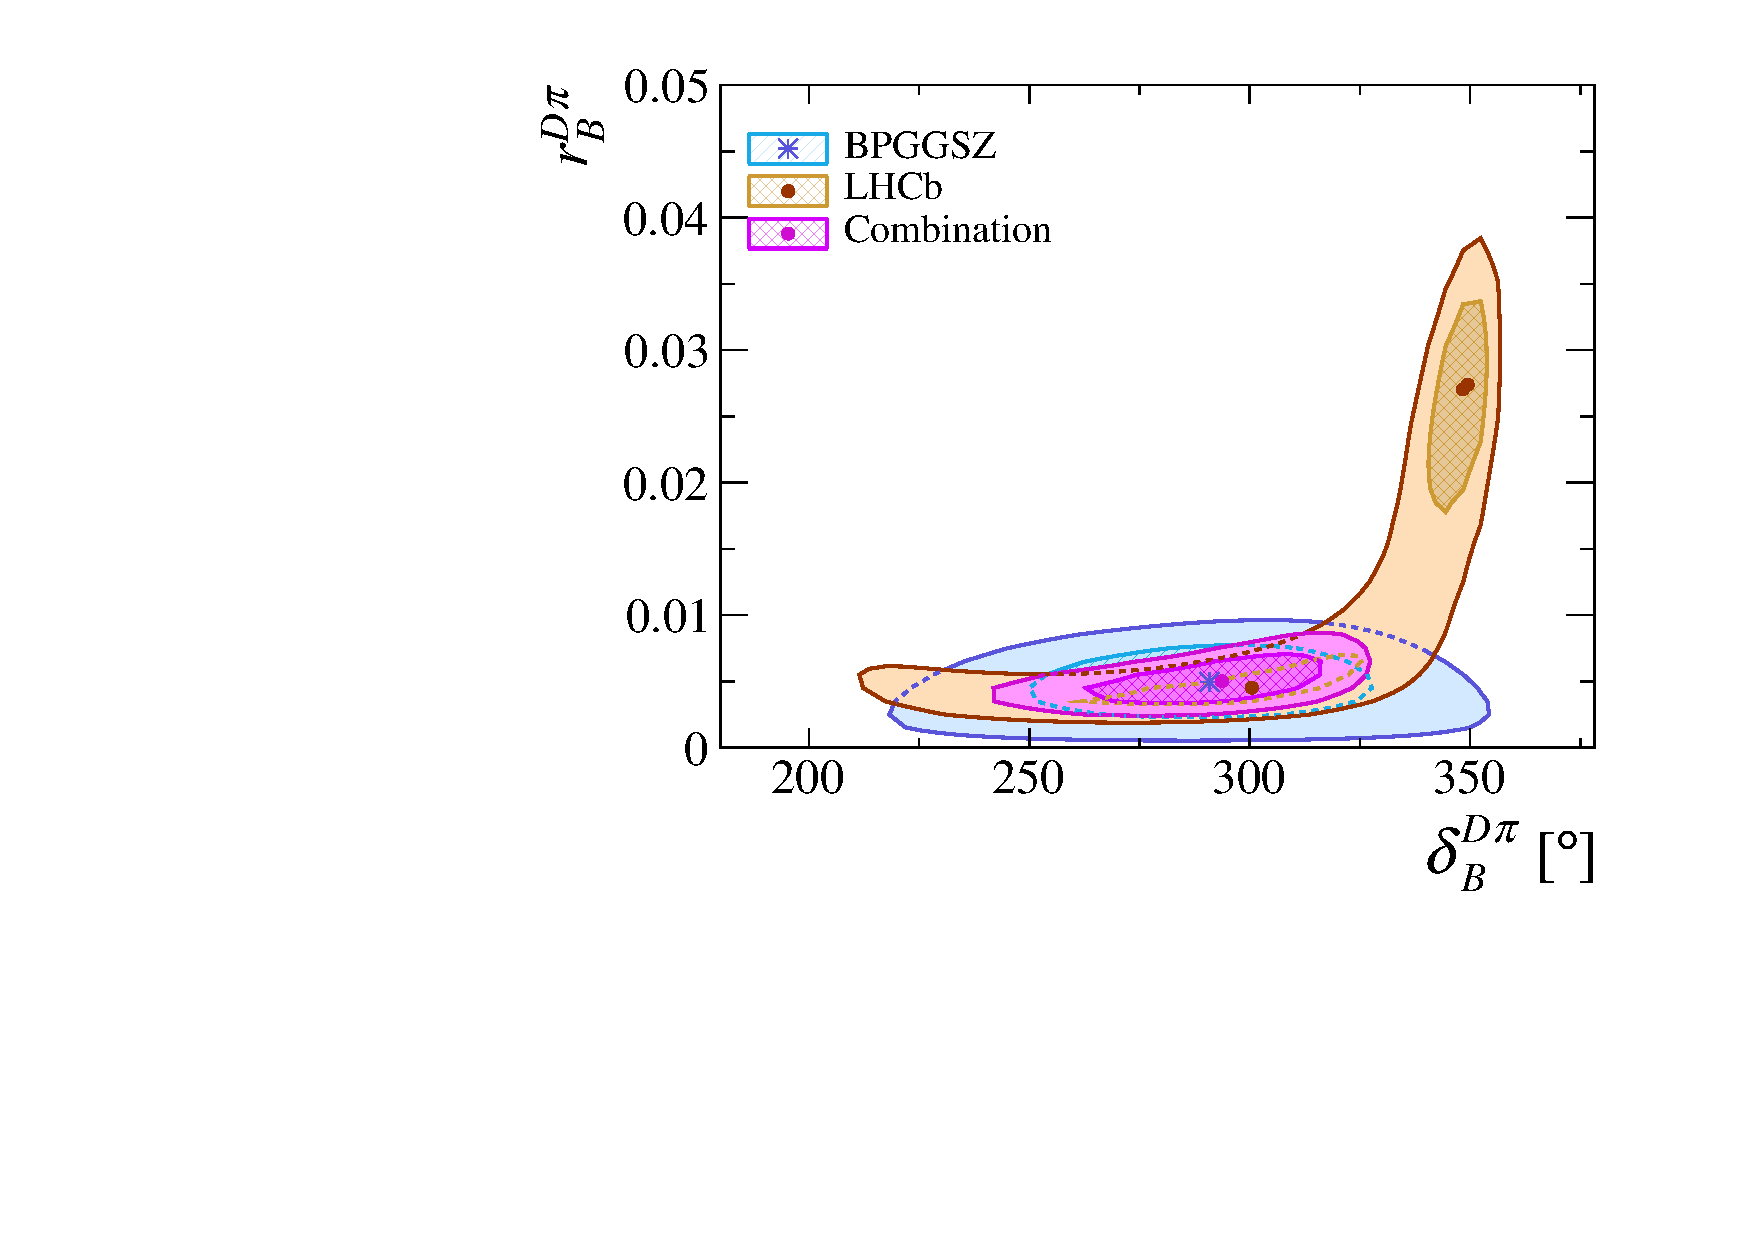
\includegraphics[width=0.47\columnwidth]{figures/analysis/interpretation/2d_d_dpi_r_dpi_vs_old_lhcb_prob.pdf}
    \caption{The 68\,\% and 95\,\% confidence regions for $(\delta_B^{\Dpi}, r_B^{\Dpi})$ obtained from the results of this measurement, in the 2016 \lhcb combination~\cite{LHCb-PAPER-2016-032}, and the combination thereof, calculated via the \texttt{PROB} method of \texttt{gammacombo}.}
    \label{fig:lhcb_dpi_comp_2d}
\end{figure}
% subsection compatibility_with_other_lhcb_measurements (end)
% section constraints_on_ (end)

% section cp_violation_and_material_interaction_of_neutral_kaons (end)